\documentclass[twoside]{book}

% Packages required by doxygen
\usepackage{fixltx2e}
\usepackage{calc}
\usepackage{doxygen}
\usepackage[export]{adjustbox} % also loads graphicx
\usepackage{graphicx}
\usepackage[utf8]{inputenc}
\usepackage{makeidx}
\usepackage{multicol}
\usepackage{multirow}
\PassOptionsToPackage{warn}{textcomp}
\usepackage{textcomp}
\usepackage[nointegrals]{wasysym}
\usepackage[table]{xcolor}

% Font selection
\usepackage[T1]{fontenc}
\usepackage[scaled=.90]{helvet}
\usepackage{courier}
\usepackage{amssymb}
\usepackage{sectsty}
\renewcommand{\familydefault}{\sfdefault}
\allsectionsfont{%
  \fontseries{bc}\selectfont%
  \color{darkgray}%
}
\renewcommand{\DoxyLabelFont}{%
  \fontseries{bc}\selectfont%
  \color{darkgray}%
}
\newcommand{\+}{\discretionary{\mbox{\scriptsize$\hookleftarrow$}}{}{}}

% Page & text layout
\usepackage{geometry}
\geometry{%
  a4paper,%
  top=2.5cm,%
  bottom=2.5cm,%
  left=2.5cm,%
  right=2.5cm%
}
\tolerance=750
\hfuzz=15pt
\hbadness=750
\setlength{\emergencystretch}{15pt}
\setlength{\parindent}{0cm}
\setlength{\parskip}{3ex plus 2ex minus 2ex}
\makeatletter
\renewcommand{\paragraph}{%
  \@startsection{paragraph}{4}{0ex}{-1.0ex}{1.0ex}{%
    \normalfont\normalsize\bfseries\SS@parafont%
  }%
}
\renewcommand{\subparagraph}{%
  \@startsection{subparagraph}{5}{0ex}{-1.0ex}{1.0ex}{%
    \normalfont\normalsize\bfseries\SS@subparafont%
  }%
}
\makeatother

% Headers & footers
\usepackage{fancyhdr}
\pagestyle{fancyplain}
\fancyhead[LE]{\fancyplain{}{\bfseries\thepage}}
\fancyhead[CE]{\fancyplain{}{}}
\fancyhead[RE]{\fancyplain{}{\bfseries\leftmark}}
\fancyhead[LO]{\fancyplain{}{\bfseries\rightmark}}
\fancyhead[CO]{\fancyplain{}{}}
\fancyhead[RO]{\fancyplain{}{\bfseries\thepage}}
\fancyfoot[LE]{\fancyplain{}{}}
\fancyfoot[CE]{\fancyplain{}{}}
\fancyfoot[RE]{\fancyplain{}{\bfseries\scriptsize Generated by Doxygen }}
\fancyfoot[LO]{\fancyplain{}{\bfseries\scriptsize Generated by Doxygen }}
\fancyfoot[CO]{\fancyplain{}{}}
\fancyfoot[RO]{\fancyplain{}{}}
\renewcommand{\footrulewidth}{0.4pt}
\renewcommand{\chaptermark}[1]{%
  \markboth{#1}{}%
}
\renewcommand{\sectionmark}[1]{%
  \markright{\thesection\ #1}%
}

% Indices & bibliography
\usepackage{natbib}
\usepackage[titles]{tocloft}
\setcounter{tocdepth}{3}
\setcounter{secnumdepth}{5}
\makeindex

% Hyperlinks (required, but should be loaded last)
\usepackage{ifpdf}
\ifpdf
  \usepackage[pdftex,pagebackref=true]{hyperref}
\else
  \usepackage[ps2pdf,pagebackref=true]{hyperref}
\fi
\hypersetup{%
  colorlinks=true,%
  linkcolor=blue,%
  citecolor=blue,%
  unicode%
}

% Custom commands
\newcommand{\clearemptydoublepage}{%
  \newpage{\pagestyle{empty}\cleardoublepage}%
}

\usepackage{caption}
\captionsetup{labelsep=space,justification=centering,font={bf},singlelinecheck=off,skip=4pt,position=top}

%===== C O N T E N T S =====

\begin{document}

% Titlepage & ToC
\hypersetup{pageanchor=false,
             bookmarksnumbered=true,
             pdfencoding=unicode
            }
\pagenumbering{alph}
\begin{titlepage}
\vspace*{7cm}
\begin{center}%
{\Large alpha\+Torrent }\\
\vspace*{1cm}
{\large Generated by Doxygen 1.8.13}\\
\end{center}
\end{titlepage}
\clearemptydoublepage
\pagenumbering{roman}
\tableofcontents
\clearemptydoublepage
\pagenumbering{arabic}
\hypersetup{pageanchor=true}

%--- Begin generated contents ---
\chapter{Namespace Index}
\section{Namespace List}
Here is a list of all documented namespaces with brief descriptions\+:\begin{DoxyCompactList}
\item\contentsline{section}{\hyperlink{namespacepwp}{pwp} }{\pageref{namespacepwp}}{}
\item\contentsline{section}{\hyperlink{namespacepwp__msg}{pwp\+\_\+msg} }{\pageref{namespacepwp__msg}}{}
\item\contentsline{section}{\hyperlink{namespacet__udp}{t\+\_\+udp} }{\pageref{namespacet__udp}}{}
\end{DoxyCompactList}

\chapter{Class Index}
\section{Class List}
Here are the classes, structs, unions and interfaces with brief descriptions\+:\begin{DoxyCompactList}
\item\contentsline{section}{\hyperlink{structt__udp_1_1announce__request}{t\+\_\+udp\+::announce\+\_\+request} }{\pageref{structt__udp_1_1announce__request}}{}
\item\contentsline{section}{\hyperlink{structt__udp_1_1announce__response}{t\+\_\+udp\+::announce\+\_\+response} }{\pageref{structt__udp_1_1announce__response}}{}
\item\contentsline{section}{\hyperlink{structbe__dict}{be\+\_\+dict} }{\pageref{structbe__dict}}{}
\item\contentsline{section}{\hyperlink{structbe__node}{be\+\_\+node} }{\pageref{structbe__node}}{}
\item\contentsline{section}{\hyperlink{structbInt}{b\+Int} }{\pageref{structbInt}}{}
\item\contentsline{section}{\hyperlink{structpwp_1_1client__state}{pwp\+::client\+\_\+state} }{\pageref{structpwp_1_1client__state}}{}
\item\contentsline{section}{\hyperlink{structt__udp_1_1connect__request}{t\+\_\+udp\+::connect\+\_\+request} }{\pageref{structt__udp_1_1connect__request}}{}
\item\contentsline{section}{\hyperlink{structt__udp_1_1connect__response}{t\+\_\+udp\+::connect\+\_\+response} }{\pageref{structt__udp_1_1connect__response}}{}
\item\contentsline{section}{\hyperlink{structpwp_1_1peer}{pwp\+::peer} }{\pageref{structpwp_1_1peer}}{}
\item\contentsline{section}{\hyperlink{classPeer}{Peer} }{\pageref{classPeer}}{}
\item\contentsline{section}{\hyperlink{structpwp_1_1peer__connection}{pwp\+::peer\+\_\+connection} }{\pageref{structpwp_1_1peer__connection}}{}
\item\contentsline{section}{\hyperlink{structpwp_1_1peer__state}{pwp\+::peer\+\_\+state} }{\pageref{structpwp_1_1peer__state}}{}
\item\contentsline{section}{\hyperlink{structfileio_1_1RequestMsg}{fileio\+::\+Request\+Msg} \\*Struct corresponding to a pwp \char`\"{}request\char`\"{} message }{\pageref{structfileio_1_1RequestMsg}}{}
\item\contentsline{section}{\hyperlink{structtorr_1_1Torrent}{torr\+::\+Torrent} \\*Struct to store all the information of a torrent }{\pageref{structtorr_1_1Torrent}}{}
\item\contentsline{section}{\hyperlink{structtorr_1_1TorrentFile}{torr\+::\+Torrent\+File} \\*Struct to store information of a file inside a torrent }{\pageref{structtorr_1_1TorrentFile}}{}
\item\contentsline{section}{\hyperlink{structtracker_1_1TParameter}{tracker\+::\+T\+Parameter} }{\pageref{structtracker_1_1TParameter}}{}
\end{DoxyCompactList}

\chapter{File Index}
\section{File List}
Here is a list of all documented files with brief descriptions\+:\begin{DoxyCompactList}
\item\contentsline{section}{lib/{\bfseries bencode.\+h} }{\pageref{bencode_8h}}{}
\item\contentsline{section}{lib/\hyperlink{filehandler_8hpp}{filehandler.\+hpp} }{\pageref{filehandler_8hpp}}{}
\item\contentsline{section}{lib/\hyperlink{peer_8h}{peer.\+h} }{\pageref{peer_8h}}{}
\item\contentsline{section}{lib/{\bfseries peer.\+hpp} }{\pageref{peer_8hpp}}{}
\item\contentsline{section}{lib/\hyperlink{pwp_8hpp}{pwp.\+hpp} }{\pageref{pwp_8hpp}}{}
\item\contentsline{section}{lib/{\bfseries rang.\+hpp} }{\pageref{rang_8hpp}}{}
\item\contentsline{section}{lib/\hyperlink{torrentparser_8hpp}{torrentparser.\+hpp} }{\pageref{torrentparser_8hpp}}{}
\item\contentsline{section}{lib/\hyperlink{tracker_8h}{tracker.\+h} }{\pageref{tracker_8h}}{}
\item\contentsline{section}{lib/\hyperlink{tracker__udp_8hpp}{tracker\+\_\+udp.\+hpp} }{\pageref{tracker__udp_8hpp}}{}
\end{DoxyCompactList}

\chapter{Namespace Documentation}
\hypertarget{namespacepwp}{}\section{pwp Namespace Reference}
\label{namespacepwp}\index{pwp@{pwp}}
\subsection*{Classes}
\begin{DoxyCompactItemize}
\item 
struct \hyperlink{structpwp_1_1client__state}{client\+\_\+state}
\item 
struct \hyperlink{structpwp_1_1peer}{peer}
\item 
struct \hyperlink{structpwp_1_1peer__connection}{peer\+\_\+connection}
\item 
struct \hyperlink{structpwp_1_1peer__state}{peer\+\_\+state}
\end{DoxyCompactItemize}
\subsection*{Typedefs}
\begin{DoxyCompactItemize}
\item 
typedef std\+::shared\+\_\+ptr$<$ std\+::vector$<$ \hyperlink{structpwp_1_1peer}{pwp\+::peer} $>$ $>$ \hyperlink{namespacepwp_ad07fa6df116b205302ad5ec172277184}{Peer\+List}
\item 
\mbox{\Hypertarget{namespacepwp_a174e8f020062fa10258b0d28f00d79ff}\label{namespacepwp_a174e8f020062fa10258b0d28f00d79ff}} 
typedef std\+::shared\+\_\+ptr$<$ std\+::vector$<$ \hyperlink{structpwp_1_1peer__connection}{pwp\+::peer\+\_\+connection} $>$ $>$ {\bfseries Peer\+Connected}
\end{DoxyCompactItemize}
\subsection*{Functions}
\begin{DoxyCompactItemize}
\item 
void \hyperlink{namespacepwp_ae8331eb5e3c98deddc6022dad92352f6}{remove\+\_\+invalid\+\_\+peer} (\hyperlink{namespacepwp_ad07fa6df116b205302ad5ec172277184}{pwp\+::\+Peer\+List} peer\+\_\+list)
\begin{DoxyCompactList}\small\item\em Find invalid peers and remove it. \end{DoxyCompactList}\item 
int \hyperlink{namespacepwp_a73acf05b954e39825a88036d5793db6b}{create\+\_\+socket} (\hyperlink{structpwp_1_1peer__connection}{pwp\+::peer\+\_\+connection} \&peer\+\_\+conn\+\_\+p)
\begin{DoxyCompactList}\small\item\em Create the socket and connect to the peer. \end{DoxyCompactList}\item 
void \hyperlink{namespacepwp_a62060bdcdc80541b0892e26fbeab1e91}{pwp\+\_\+protocol\+\_\+manager} (\hyperlink{structpwp_1_1peer}{pwp\+::peer} peer\+\_\+, const std\+::vector$<$ uint8\+\_\+t $>$ \&handshake, const char $\ast$info\+\_\+hash, \hyperlink{structtorr_1_1Torrent}{Torrent} \&torrent)
\begin{DoxyCompactList}\small\item\em Manager of the entire P\+WP protocol. \end{DoxyCompactList}\item 
void \hyperlink{namespacepwp_a6062876f4d4d4d6ee19341a79a797864}{build\+\_\+handshake} (char $\ast$info\+\_\+hash, std\+::vector$<$ uint8\+\_\+t $>$ \&handshake)
\item 
int \hyperlink{namespacepwp_a851ddc0e8fb2eb0a86317cc944c4a927}{send\+\_\+handshake} (\hyperlink{structpwp_1_1peer__connection}{pwp\+::peer\+\_\+connection} \&peerc\+\_\+t, const std\+::vector$<$ uint8\+\_\+t $>$ handshake, std\+::vector$<$ uint8\+\_\+t $>$ \&response)
\item 
void \hyperlink{namespacepwp_ada6a8613896dbbfd6fba63b17d51684c}{get\+\_\+peer\+\_\+id} (string $\ast$id)
\begin{DoxyCompactList}\small\item\em Put into \char`\"{}id\char`\"{} the string that conrespond to the client ID. \end{DoxyCompactList}\item 
int \hyperlink{namespacepwp_a58c780495f2139a56b95662dc7c0345f}{verify\+\_\+handshake} (const vector$<$ uint8\+\_\+t $>$ handshake, size\+\_\+t len, const \hyperlink{structpwp_1_1peer}{pwp\+::peer} t\+\_\+peer, const char $\ast$info\+\_\+hash)
\item 
\mbox{\Hypertarget{namespacepwp_ab82c0d015f6ba23e766c4b942a125b5f}\label{namespacepwp_ab82c0d015f6ba23e766c4b942a125b5f}} 
void {\bfseries manage\+\_\+peer\+\_\+connection} (\hyperlink{namespacepwp_ad07fa6df116b205302ad5ec172277184}{pwp\+::\+Peer\+List} peer\+\_\+list, char $\ast$info\+\_\+hash)
\item 
\mbox{\Hypertarget{namespacepwp_a5f03cde749af88a393c999545830b192}\label{namespacepwp_a5f03cde749af88a393c999545830b192}} 
void {\bfseries get\+\_\+peer\+\_\+id} (std\+::string $\ast$id)
\item 
\mbox{\Hypertarget{namespacepwp_ae2eeca61e271fabff5fa45308396009e}\label{namespacepwp_ae2eeca61e271fabff5fa45308396009e}} 
void {\bfseries handshake\+\_\+request\+\_\+manager} (const std\+::array$<$ char, 256 $>$ \&handshake, const \hyperlink{structpwp_1_1peer}{pwp\+::peer} t\+\_\+peer, const char $\ast$info\+\_\+hash, pwp\+::\+Peer\+Connected valid\+\_\+peer)
\item 
\mbox{\Hypertarget{namespacepwp_aed118903b8345e62507ade49c6032d32}\label{namespacepwp_aed118903b8345e62507ade49c6032d32}} 
int {\bfseries verify\+\_\+handshake} (const std\+::vector$<$ uint8\+\_\+t $>$ handshake, size\+\_\+t len, const \hyperlink{structpwp_1_1peer}{pwp\+::peer} t\+\_\+peer, const char $\ast$info\+\_\+hash)
\end{DoxyCompactItemize}


\subsection{Detailed Description}
Namespace used to define all peer\textquotesingle{}s related data and P\+WP protocol 

\subsection{Typedef Documentation}
\mbox{\Hypertarget{namespacepwp_ad07fa6df116b205302ad5ec172277184}\label{namespacepwp_ad07fa6df116b205302ad5ec172277184}} 
\index{pwp@{pwp}!Peer\+List@{Peer\+List}}
\index{Peer\+List@{Peer\+List}!pwp@{pwp}}
\subsubsection{\texorpdfstring{Peer\+List}{PeerList}}
{\footnotesize\ttfamily typedef std\+::shared\+\_\+ptr$<$std\+::vector$<$\hyperlink{structpwp_1_1peer}{pwp\+::peer}$>$ $>$ \hyperlink{namespacepwp_ad07fa6df116b205302ad5ec172277184}{pwp\+::\+Peer\+List}}

peer list extracted from tracker 

\subsection{Function Documentation}
\mbox{\Hypertarget{namespacepwp_a6062876f4d4d4d6ee19341a79a797864}\label{namespacepwp_a6062876f4d4d4d6ee19341a79a797864}} 
\index{pwp@{pwp}!build\+\_\+handshake@{build\+\_\+handshake}}
\index{build\+\_\+handshake@{build\+\_\+handshake}!pwp@{pwp}}
\subsubsection{\texorpdfstring{build\+\_\+handshake()}{build\_handshake()}}
{\footnotesize\ttfamily void pwp\+::build\+\_\+handshake (\begin{DoxyParamCaption}\item[{char $\ast$}]{info\+\_\+hash,  }\item[{std\+::vector$<$ uint8\+\_\+t $>$ \&}]{handshake }\end{DoxyParamCaption})}

Create the handshake for a file


\begin{DoxyParams}{Parameters}
{\em info\+\_\+hash} & the info\+\_\+hash of the file \\
\hline
{\em handshake} & the destination array for the handshake \\
\hline
\end{DoxyParams}
\mbox{\Hypertarget{namespacepwp_a73acf05b954e39825a88036d5793db6b}\label{namespacepwp_a73acf05b954e39825a88036d5793db6b}} 
\index{pwp@{pwp}!create\+\_\+socket@{create\+\_\+socket}}
\index{create\+\_\+socket@{create\+\_\+socket}!pwp@{pwp}}
\subsubsection{\texorpdfstring{create\+\_\+socket()}{create\_socket()}}
{\footnotesize\ttfamily int pwp\+::create\+\_\+socket (\begin{DoxyParamCaption}\item[{\hyperlink{structpwp_1_1peer__connection}{pwp\+::peer\+\_\+connection} \&}]{peer\+\_\+conn\+\_\+p }\end{DoxyParamCaption})}



Create the socket and connect to the peer. 

\tabulinesep=1mm
\begin{longtabu} spread 0pt [c]{*{2}{|X[-1]}|}
\hline
\rowcolor{\tableheadbgcolor}\textbf{ Error Code }&\textbf{ Meaning  }\\\cline{1-2}
\endfirsthead
\hline
\endfoot
\hline
\rowcolor{\tableheadbgcolor}\textbf{ Error Code }&\textbf{ Meaning  }\\\cline{1-2}
\endhead
-\/1 &Connection Closed \\\cline{1-2}
-\/2 &Generic Error (see the output) \\\cline{1-2}
-\/3 &Invalid Address \\\cline{1-2}
\end{longtabu}



\begin{DoxyParams}{Parameters}
{\em \hyperlink{structpwp_1_1peer__connection}{peer\+\_\+connection}} & \\
\hline
\end{DoxyParams}
\mbox{\Hypertarget{namespacepwp_ada6a8613896dbbfd6fba63b17d51684c}\label{namespacepwp_ada6a8613896dbbfd6fba63b17d51684c}} 
\index{pwp@{pwp}!get\+\_\+peer\+\_\+id@{get\+\_\+peer\+\_\+id}}
\index{get\+\_\+peer\+\_\+id@{get\+\_\+peer\+\_\+id}!pwp@{pwp}}
\subsubsection{\texorpdfstring{get\+\_\+peer\+\_\+id()}{get\_peer\_id()}}
{\footnotesize\ttfamily void pwp\+::get\+\_\+peer\+\_\+id (\begin{DoxyParamCaption}\item[{string $\ast$}]{id }\end{DoxyParamCaption})}



Put into \char`\"{}id\char`\"{} the string that conrespond to the client ID. 

Find a new way to generate the ID\+:
\begin{DoxyEnumerate}
\item Using M\+AC address.
\item Initially random and then writtend o a file.
\end{DoxyEnumerate}


\begin{DoxyParams}{Parameters}
{\em id} & A pointer to the string that will contains the Peer-\/\+ID \\
\hline
\end{DoxyParams}
\mbox{\Hypertarget{namespacepwp_a62060bdcdc80541b0892e26fbeab1e91}\label{namespacepwp_a62060bdcdc80541b0892e26fbeab1e91}} 
\index{pwp@{pwp}!pwp\+\_\+protocol\+\_\+manager@{pwp\+\_\+protocol\+\_\+manager}}
\index{pwp\+\_\+protocol\+\_\+manager@{pwp\+\_\+protocol\+\_\+manager}!pwp@{pwp}}
\subsubsection{\texorpdfstring{pwp\+\_\+protocol\+\_\+manager()}{pwp\_protocol\_manager()}}
{\footnotesize\ttfamily void pwp\+::pwp\+\_\+protocol\+\_\+manager (\begin{DoxyParamCaption}\item[{\hyperlink{structpwp_1_1peer}{pwp\+::peer}}]{peer\+\_\+,  }\item[{const std\+::vector$<$ uint8\+\_\+t $>$ \&}]{handshake,  }\item[{const char $\ast$}]{info\+\_\+hash,  }\item[{\hyperlink{structtorr_1_1Torrent}{Torrent} \&}]{torrent }\end{DoxyParamCaption})}



Manager of the entire P\+WP protocol. 

This is the manager of the entire peer comunication. After creating the socket the handshake is sended. The received handshake is then checked and if it\textquotesingle{}s correct the routine starts.


\begin{DoxyEnumerate}
\item Send Interested Message
\item Send Unchocked Message
\item Start Keep-\/\+Alive Routine
\item Wait (asynchronously) for messages
\item Loop and send appropriate messages
\end{DoxyEnumerate}

\begin{DoxyRefDesc}{Bug}
\item[\hyperlink{bug__bug000001}{Bug}]No timeout control is performed so if there is a dead peer that does not respond the software blocks until the default SO timeout is reacher (tipically 2 minutes).\end{DoxyRefDesc}



\begin{DoxyParams}{Parameters}
{\em peer\+\_\+} & The peer on which execute the protocol \\
\hline
{\em handshake} & The initial handshake to send \\
\hline
{\em info\+\_\+hash} & The torrent file info\+\_\+hash \\
\hline
{\em torrent} & The struct containing all torrent information \\
\hline
\end{DoxyParams}
\mbox{\Hypertarget{namespacepwp_ae8331eb5e3c98deddc6022dad92352f6}\label{namespacepwp_ae8331eb5e3c98deddc6022dad92352f6}} 
\index{pwp@{pwp}!remove\+\_\+invalid\+\_\+peer@{remove\+\_\+invalid\+\_\+peer}}
\index{remove\+\_\+invalid\+\_\+peer@{remove\+\_\+invalid\+\_\+peer}!pwp@{pwp}}
\subsubsection{\texorpdfstring{remove\+\_\+invalid\+\_\+peer()}{remove\_invalid\_peer()}}
{\footnotesize\ttfamily void pwp\+::remove\+\_\+invalid\+\_\+peer (\begin{DoxyParamCaption}\item[{\hyperlink{namespacepwp_ad07fa6df116b205302ad5ec172277184}{pwp\+::\+Peer\+List}}]{peer\+\_\+list }\end{DoxyParamCaption})}



Find invalid peers and remove it. 


\begin{DoxyParams}{Parameters}
{\em peer\+\_\+list} & \\
\hline
\end{DoxyParams}
\mbox{\Hypertarget{namespacepwp_a851ddc0e8fb2eb0a86317cc944c4a927}\label{namespacepwp_a851ddc0e8fb2eb0a86317cc944c4a927}} 
\index{pwp@{pwp}!send\+\_\+handshake@{send\+\_\+handshake}}
\index{send\+\_\+handshake@{send\+\_\+handshake}!pwp@{pwp}}
\subsubsection{\texorpdfstring{send\+\_\+handshake()}{send\_handshake()}}
{\footnotesize\ttfamily int pwp\+::send\+\_\+handshake (\begin{DoxyParamCaption}\item[{\hyperlink{structpwp_1_1peer__connection}{pwp\+::peer\+\_\+connection} \&}]{peerc\+\_\+t,  }\item[{const std\+::vector$<$ uint8\+\_\+t $>$}]{handshake,  }\item[{std\+::vector$<$ uint8\+\_\+t $>$ \&}]{response }\end{DoxyParamCaption})}

Contact the peer with handshake and download the response

\tabulinesep=1mm
\begin{longtabu} spread 0pt [c]{*{2}{|X[-1]}|}
\hline
\rowcolor{\tableheadbgcolor}\textbf{ Error code }&\textbf{ Meaning  }\\\cline{1-2}
\endfirsthead
\hline
\endfoot
\hline
\rowcolor{\tableheadbgcolor}\textbf{ Error code }&\textbf{ Meaning  }\\\cline{1-2}
\endhead
-\/1 &Unimplemented. \\\cline{1-2}
-\/2 &Socket Error. \\\cline{1-2}
-\/3 &Invalid IP Address. \\\cline{1-2}
\end{longtabu}



\begin{DoxyParams}{Parameters}
{\em t\+\_\+peer} & the peer to contact \\
\hline
{\em handshake} & the handshake to send \\
\hline
{\em response} & a pointer to an array used to store the response\\
\hline
\end{DoxyParams}
\begin{DoxyReturn}{Returns}
0 on success, $<$ 0 on failure 
\end{DoxyReturn}
\mbox{\Hypertarget{namespacepwp_a58c780495f2139a56b95662dc7c0345f}\label{namespacepwp_a58c780495f2139a56b95662dc7c0345f}} 
\index{pwp@{pwp}!verify\+\_\+handshake@{verify\+\_\+handshake}}
\index{verify\+\_\+handshake@{verify\+\_\+handshake}!pwp@{pwp}}
\subsubsection{\texorpdfstring{verify\+\_\+handshake()}{verify\_handshake()}}
{\footnotesize\ttfamily int pwp\+::verify\+\_\+handshake (\begin{DoxyParamCaption}\item[{const vector$<$ uint8\+\_\+t $>$}]{handshake,  }\item[{size\+\_\+t}]{len,  }\item[{const \hyperlink{structpwp_1_1peer}{pwp\+::peer}}]{t\+\_\+peer,  }\item[{const char $\ast$}]{info\+\_\+hash }\end{DoxyParamCaption})}

Verify if an handshake (received) is correct

\tabulinesep=1mm
\begin{longtabu} spread 0pt [c]{*{2}{|X[-1]}|}
\hline
\rowcolor{\tableheadbgcolor}\textbf{ Error Code }&\textbf{ Meaning  }\\\cline{1-2}
\endfirsthead
\hline
\endfoot
\hline
\rowcolor{\tableheadbgcolor}\textbf{ Error Code }&\textbf{ Meaning  }\\\cline{1-2}
\endhead
-\/1 &First byte is not 19 \\\cline{1-2}
-\/2 &Invalid protocol string \\\cline{1-2}
-\/3 &Info hash does not match (with the one sended) \\\cline{1-2}
-\/4 &Peer ID does not match (Bypassed) \\\cline{1-2}
\end{longtabu}
\begin{DoxyWarning}{Warning}
The comparison of the {\itshape peer-\/\+ID} often fail so it\textquotesingle{}s skipped (no return -\/4)
\end{DoxyWarning}

\begin{DoxyParams}{Parameters}
{\em handshake} & \+: the handshake to check \\
\hline
{\em t\+\_\+peer} & \+: the peer who sended the handshake \\
\hline
{\em info\+\_\+hash} & \+: the info\+\_\+hash of the file \\
\hline
\end{DoxyParams}
If the initiator of the connection receives a handshake in which the peer\+\_\+id does not match the expected peerid, then the initiator is expected to drop the connection. Note that the initiator presumably received the peer information from the tracker, which includes the peer\+\_\+id that was registered by the peer. The peer\+\_\+id from the tracker and in the handshake are expected to match.
\hypertarget{namespacepwp__msg}{}\section{pwp\+\_\+msg Namespace Reference}
\label{namespacepwp__msg}\index{pwp\+\_\+msg@{pwp\+\_\+msg}}
\subsection*{Enumerations}
\begin{DoxyCompactItemize}
\item 
enum \hyperlink{namespacepwp__msg_a0b9a29508f00a30e5138d2b78f4b1daf}{msg\+\_\+id} \{ \newline
\hyperlink{namespacepwp__msg_a0b9a29508f00a30e5138d2b78f4b1dafae1d8b3754d66ec7fcad827fb54eaeea2}{chocked} = 0x00, 
\hyperlink{namespacepwp__msg_a0b9a29508f00a30e5138d2b78f4b1dafa55689e288bf71e7737faaf385b1c528b}{unchocked} = 0x01, 
{\bfseries interested} = 0x02, 
{\bfseries not\+\_\+interested} = 0x03, 
\newline
{\bfseries have} = 0x04, 
\hyperlink{namespacepwp__msg_a0b9a29508f00a30e5138d2b78f4b1dafac3a2343a7b67a371e241ae2184bfe9cd}{bitfield} = 0x05, 
{\bfseries request} = 0x06, 
{\bfseries piece} = 0x07, 
\newline
{\bfseries cancel} = 0x08, 
{\bfseries port} = 0x09
 \}
\end{DoxyCompactItemize}
\subsection*{Functions}
\begin{DoxyCompactItemize}
\item 
void \hyperlink{namespacepwp__msg_a9a577f5a53b823d83bb4694f1ebf141e}{send\+\_\+keep\+\_\+alive} (const \hyperlink{structpwp_1_1peer__connection}{pwp\+::peer\+\_\+connection} \&peer\+\_\+c, boost\+::asio\+::deadline\+\_\+timer \&timer)
\item 
void \hyperlink{namespacepwp__msg_a30c14bc06a8bb851ca79781cb9686b4f}{enable\+\_\+keep\+\_\+alive\+\_\+message} (\hyperlink{structpwp_1_1peer__connection}{pwp\+::peer\+\_\+connection} \&peer\+\_\+c)
\item 
int \hyperlink{namespacepwp__msg_aca807c6281879abef952f8feecccb6e8}{send\+\_\+msg} (\hyperlink{structpwp_1_1peer__connection}{pwp\+::peer\+\_\+connection} \&peer\+\_\+c, std\+::vector$<$ uint8\+\_\+t $>$ msg)
\begin{DoxyCompactList}\small\item\em Send {\ttfamily msg} to the peer specified in {\ttfamily peer\+\_\+c} \end{DoxyCompactList}\item 
\mbox{\Hypertarget{namespacepwp__msg_a529a3db7938ccfaab85579d58e24061e}\label{namespacepwp__msg_a529a3db7938ccfaab85579d58e24061e}} 
std\+::vector$<$ uint8\+\_\+t $>$ {\bfseries craft\+\_\+have\+\_\+msg} (int piece\+\_\+index)
\item 
\mbox{\Hypertarget{namespacepwp__msg_a2dcbe5fbe0eeca8910340f4978ee4235}\label{namespacepwp__msg_a2dcbe5fbe0eeca8910340f4978ee4235}} 
std\+::vector$<$ uint8\+\_\+t $>$ {\bfseries make\+\_\+request\+\_\+msg} (\hyperlink{structRequestMsg}{Request\+Msg} request)
\item 
\mbox{\Hypertarget{namespacepwp__msg_aa9cc2ccac70638ed59075f27f938b8ec}\label{namespacepwp__msg_aa9cc2ccac70638ed59075f27f938b8ec}} 
int {\bfseries get\+\_\+bitfield} (\hyperlink{structpwp_1_1peer__connection}{pwp\+::peer\+\_\+connection} \&peer\+\_\+c, \hyperlink{structTorrent}{Torrent} \&torrent)
\item 
\mbox{\Hypertarget{namespacepwp__msg_aec35de04a2f2d9cb6abdd777917cfaae}\label{namespacepwp__msg_aec35de04a2f2d9cb6abdd777917cfaae}} 
void {\bfseries read\+\_\+msg\+\_\+handler} (std\+::vector$<$ uint8\+\_\+t $>$ \&response, \hyperlink{structpwp_1_1peer__connection}{pwp\+::peer\+\_\+connection} \&peer\+\_\+c, \hyperlink{structTorrent}{Torrent} \&torrent, bool \&dead\+\_\+peer, boost\+::asio\+::deadline\+\_\+timer \&timer\+\_\+, const boost\+::system\+::error\+\_\+code \&error, size\+\_\+t bytes\+\_\+read)
\item 
\mbox{\Hypertarget{namespacepwp__msg_ab578b213d293636d33efc24382f16b25}\label{namespacepwp__msg_ab578b213d293636d33efc24382f16b25}} 
int {\bfseries sender} (\hyperlink{structpwp_1_1peer__connection}{pwp\+::peer\+\_\+connection} \&peer\+\_\+conn, \hyperlink{structTorrent}{Torrent} \&torrent, int \&old\+\_\+begin)
\end{DoxyCompactItemize}
\subsection*{Variables}
\begin{DoxyCompactItemize}
\item 
\mbox{\Hypertarget{namespacepwp__msg_ae962e65b1871714756b6aeb4722a8caf}\label{namespacepwp__msg_ae962e65b1871714756b6aeb4722a8caf}} 
enum \hyperlink{namespacepwp__msg_a0b9a29508f00a30e5138d2b78f4b1daf}{pwp\+\_\+msg\+::msg\+\_\+id} {\bfseries Peer\+List}
\item 
const std\+::vector$<$ uint8\+\_\+t $>$ \hyperlink{namespacepwp__msg_a695ee2efb59a7c258559f19440fe6998}{choke\+\_\+msg} = \{0,0,0,1,0\}
\item 
const std\+::vector$<$ uint8\+\_\+t $>$ \hyperlink{namespacepwp__msg_acdc5eb698534e84a15db0e061c511e7c}{unchoke\+\_\+msg} = \{0,0,0,1,1\}
\item 
const std\+::vector$<$ uint8\+\_\+t $>$ \hyperlink{namespacepwp__msg_afc68b17ce131c52fa0beb0cc7185778b}{interested\+\_\+msg} = \{0,0,0,1,2\}
\item 
const std\+::vector$<$ uint8\+\_\+t $>$ \hyperlink{namespacepwp__msg_a16a5f22f784d872342a82af9f6b77830}{non\+\_\+interested\+\_\+msg} = \{0,0,0,1,3\}
\end{DoxyCompactItemize}


\subsection{Detailed Description}
This namespace contains all the function that are related to the messages of the P\+WP Protocol 

\subsection{Enumeration Type Documentation}
\mbox{\Hypertarget{namespacepwp__msg_a0b9a29508f00a30e5138d2b78f4b1daf}\label{namespacepwp__msg_a0b9a29508f00a30e5138d2b78f4b1daf}} 
\index{pwp\+\_\+msg@{pwp\+\_\+msg}!msg\+\_\+id@{msg\+\_\+id}}
\index{msg\+\_\+id@{msg\+\_\+id}!pwp\+\_\+msg@{pwp\+\_\+msg}}
\subsubsection{\texorpdfstring{msg\+\_\+id}{msg\_id}}
{\footnotesize\ttfamily enum \hyperlink{namespacepwp__msg_a0b9a29508f00a30e5138d2b78f4b1daf}{pwp\+\_\+msg\+::msg\+\_\+id}}

P\+WP Message ID \begin{DoxyEnumFields}{Enumerator}
\raisebox{\heightof{T}}[0pt][0pt]{\index{chocked@{chocked}!pwp\+\_\+msg@{pwp\+\_\+msg}}\index{pwp\+\_\+msg@{pwp\+\_\+msg}!chocked@{chocked}}}\mbox{\Hypertarget{namespacepwp__msg_a0b9a29508f00a30e5138d2b78f4b1dafae1d8b3754d66ec7fcad827fb54eaeea2}\label{namespacepwp__msg_a0b9a29508f00a30e5138d2b78f4b1dafae1d8b3754d66ec7fcad827fb54eaeea2}} 
chocked&Chocked state \\
\hline

\raisebox{\heightof{T}}[0pt][0pt]{\index{unchocked@{unchocked}!pwp\+\_\+msg@{pwp\+\_\+msg}}\index{pwp\+\_\+msg@{pwp\+\_\+msg}!unchocked@{unchocked}}}\mbox{\Hypertarget{namespacepwp__msg_a0b9a29508f00a30e5138d2b78f4b1dafa55689e288bf71e7737faaf385b1c528b}\label{namespacepwp__msg_a0b9a29508f00a30e5138d2b78f4b1dafa55689e288bf71e7737faaf385b1c528b}} 
unchocked&Unchocked state \\
\hline

\raisebox{\heightof{T}}[0pt][0pt]{\index{bitfield@{bitfield}!pwp\+\_\+msg@{pwp\+\_\+msg}}\index{pwp\+\_\+msg@{pwp\+\_\+msg}!bitfield@{bitfield}}}\mbox{\Hypertarget{namespacepwp__msg_a0b9a29508f00a30e5138d2b78f4b1dafac3a2343a7b67a371e241ae2184bfe9cd}\label{namespacepwp__msg_a0b9a29508f00a30e5138d2b78f4b1dafac3a2343a7b67a371e241ae2184bfe9cd}} 
bitfield&Bitfield sended/received \\
\hline

\end{DoxyEnumFields}


\subsection{Function Documentation}
\mbox{\Hypertarget{namespacepwp__msg_a30c14bc06a8bb851ca79781cb9686b4f}\label{namespacepwp__msg_a30c14bc06a8bb851ca79781cb9686b4f}} 
\index{pwp\+\_\+msg@{pwp\+\_\+msg}!enable\+\_\+keep\+\_\+alive\+\_\+message@{enable\+\_\+keep\+\_\+alive\+\_\+message}}
\index{enable\+\_\+keep\+\_\+alive\+\_\+message@{enable\+\_\+keep\+\_\+alive\+\_\+message}!pwp\+\_\+msg@{pwp\+\_\+msg}}
\subsubsection{\texorpdfstring{enable\+\_\+keep\+\_\+alive\+\_\+message()}{enable\_keep\_alive\_message()}}
{\footnotesize\ttfamily void pwp\+\_\+msg\+::enable\+\_\+keep\+\_\+alive\+\_\+message (\begin{DoxyParamCaption}\item[{\hyperlink{structpwp_1_1peer__connection}{pwp\+::peer\+\_\+connection} \&}]{peer\+\_\+c }\end{DoxyParamCaption})}

Start the timer that each K\+E\+E\+P\+\_\+\+A\+L\+I\+V\+E\+\_\+\+T\+I\+ME send a Keep-\/alive request


\begin{DoxyParams}{Parameters}
{\em peer\+\_\+c} & The peer\textquotesingle{}s connection structure \\
\hline
\end{DoxyParams}
\mbox{\Hypertarget{namespacepwp__msg_a9a577f5a53b823d83bb4694f1ebf141e}\label{namespacepwp__msg_a9a577f5a53b823d83bb4694f1ebf141e}} 
\index{pwp\+\_\+msg@{pwp\+\_\+msg}!send\+\_\+keep\+\_\+alive@{send\+\_\+keep\+\_\+alive}}
\index{send\+\_\+keep\+\_\+alive@{send\+\_\+keep\+\_\+alive}!pwp\+\_\+msg@{pwp\+\_\+msg}}
\subsubsection{\texorpdfstring{send\+\_\+keep\+\_\+alive()}{send\_keep\_alive()}}
{\footnotesize\ttfamily void pwp\+\_\+msg\+::send\+\_\+keep\+\_\+alive (\begin{DoxyParamCaption}\item[{const \hyperlink{structpwp_1_1peer__connection}{pwp\+::peer\+\_\+connection} \&}]{peer\+\_\+c,  }\item[{boost\+::asio\+::deadline\+\_\+timer \&}]{timer }\end{DoxyParamCaption})}

Handler that is executed every K\+E\+E\+P\+\_\+\+A\+L\+I\+V\+E\+\_\+\+T\+I\+ME and send a keep-\/alive message.

If the peer\+\_\+c\textquotesingle{}s socket is closed, then the periodic routine is stopped by calling.~\newline
 {\ttfamily timer.\+cancel()} So the handler is calcelled from \hyperlink{pwp_8hpp_a7efe93eb3d4e0f0c9ab96fa5ae443fcd}{\+\_\+io\+\_\+service}


\begin{DoxyParams}{Parameters}
{\em peer\+\_\+c} & The peer connection structure. \\
\hline
{\em timer} & The deadline\+\_\+timer that call the handler. \\
\hline
\end{DoxyParams}
\mbox{\Hypertarget{namespacepwp__msg_aca807c6281879abef952f8feecccb6e8}\label{namespacepwp__msg_aca807c6281879abef952f8feecccb6e8}} 
\index{pwp\+\_\+msg@{pwp\+\_\+msg}!send\+\_\+msg@{send\+\_\+msg}}
\index{send\+\_\+msg@{send\+\_\+msg}!pwp\+\_\+msg@{pwp\+\_\+msg}}
\subsubsection{\texorpdfstring{send\+\_\+msg()}{send\_msg()}}
{\footnotesize\ttfamily int pwp\+\_\+msg\+::send\+\_\+msg (\begin{DoxyParamCaption}\item[{\hyperlink{structpwp_1_1peer__connection}{pwp\+::peer\+\_\+connection} \&}]{peer\+\_\+c,  }\item[{std\+::vector$<$ uint8\+\_\+t $>$}]{msg }\end{DoxyParamCaption})}



Send {\ttfamily msg} to the peer specified in {\ttfamily peer\+\_\+c} 

Error code list

\tabulinesep=1mm
\begin{longtabu} spread 0pt [c]{*{2}{|X[-1]}|}
\hline
\rowcolor{\tableheadbgcolor}\textbf{ Error Code }&\textbf{ Explaination  }\\\cline{1-2}
\endfirsthead
\hline
\endfoot
\hline
\rowcolor{\tableheadbgcolor}\textbf{ Error Code }&\textbf{ Explaination  }\\\cline{1-2}
\endhead
-\/1 &Invalid Address \\\cline{1-2}
-\/2 &Cannot open socket \\\cline{1-2}
-\/3 &Connection closed \\\cline{1-2}
-\/4 &Exception (see the output) \\\cline{1-2}
\end{longtabu}

\begin{DoxyParams}{Parameters}
{\em peer\+\_\+c} & \hyperlink{classPeer}{Peer} connection structure \\
\hline
{\em msg} & Message to send \\
\hline
\end{DoxyParams}
\begin{DoxyReturn}{Returns}
0 on success, $<$0 otherwise 
\end{DoxyReturn}


\subsection{Variable Documentation}
\mbox{\Hypertarget{namespacepwp__msg_a695ee2efb59a7c258559f19440fe6998}\label{namespacepwp__msg_a695ee2efb59a7c258559f19440fe6998}} 
\index{pwp\+\_\+msg@{pwp\+\_\+msg}!choke\+\_\+msg@{choke\+\_\+msg}}
\index{choke\+\_\+msg@{choke\+\_\+msg}!pwp\+\_\+msg@{pwp\+\_\+msg}}
\subsubsection{\texorpdfstring{choke\+\_\+msg}{choke\_msg}}
{\footnotesize\ttfamily const std\+::vector$<$uint8\+\_\+t$>$ pwp\+\_\+msg\+::choke\+\_\+msg = \{0,0,0,1,0\}}

Default chocked message \mbox{\Hypertarget{namespacepwp__msg_afc68b17ce131c52fa0beb0cc7185778b}\label{namespacepwp__msg_afc68b17ce131c52fa0beb0cc7185778b}} 
\index{pwp\+\_\+msg@{pwp\+\_\+msg}!interested\+\_\+msg@{interested\+\_\+msg}}
\index{interested\+\_\+msg@{interested\+\_\+msg}!pwp\+\_\+msg@{pwp\+\_\+msg}}
\subsubsection{\texorpdfstring{interested\+\_\+msg}{interested\_msg}}
{\footnotesize\ttfamily const std\+::vector$<$uint8\+\_\+t$>$ pwp\+\_\+msg\+::interested\+\_\+msg = \{0,0,0,1,2\}}

Default interested message \mbox{\Hypertarget{namespacepwp__msg_a16a5f22f784d872342a82af9f6b77830}\label{namespacepwp__msg_a16a5f22f784d872342a82af9f6b77830}} 
\index{pwp\+\_\+msg@{pwp\+\_\+msg}!non\+\_\+interested\+\_\+msg@{non\+\_\+interested\+\_\+msg}}
\index{non\+\_\+interested\+\_\+msg@{non\+\_\+interested\+\_\+msg}!pwp\+\_\+msg@{pwp\+\_\+msg}}
\subsubsection{\texorpdfstring{non\+\_\+interested\+\_\+msg}{non\_interested\_msg}}
{\footnotesize\ttfamily const std\+::vector$<$uint8\+\_\+t$>$ pwp\+\_\+msg\+::non\+\_\+interested\+\_\+msg = \{0,0,0,1,3\}}

Default non interested message \mbox{\Hypertarget{namespacepwp__msg_acdc5eb698534e84a15db0e061c511e7c}\label{namespacepwp__msg_acdc5eb698534e84a15db0e061c511e7c}} 
\index{pwp\+\_\+msg@{pwp\+\_\+msg}!unchoke\+\_\+msg@{unchoke\+\_\+msg}}
\index{unchoke\+\_\+msg@{unchoke\+\_\+msg}!pwp\+\_\+msg@{pwp\+\_\+msg}}
\subsubsection{\texorpdfstring{unchoke\+\_\+msg}{unchoke\_msg}}
{\footnotesize\ttfamily const std\+::vector$<$uint8\+\_\+t$>$ pwp\+\_\+msg\+::unchoke\+\_\+msg = \{0,0,0,1,1\}}

Default unchocked message 
\hypertarget{namespacet__udp}{}\section{t\+\_\+udp Namespace Reference}
\label{namespacet__udp}\index{t\+\_\+udp@{t\+\_\+udp}}
\subsection*{Classes}
\begin{DoxyCompactItemize}
\item 
struct \hyperlink{structt__udp_1_1announce__request}{announce\+\_\+request}
\item 
struct \hyperlink{structt__udp_1_1announce__response}{announce\+\_\+response}
\item 
struct \hyperlink{structt__udp_1_1connect__request}{connect\+\_\+request}
\item 
struct \hyperlink{structt__udp_1_1connect__response}{connect\+\_\+response}
\end{DoxyCompactItemize}
\subsection*{Enumerations}
\begin{DoxyCompactItemize}
\item 
\mbox{\Hypertarget{namespacet__udp_a6196aec9debc020a36ee358692339614}\label{namespacet__udp_a6196aec9debc020a36ee358692339614}} 
enum {\bfseries action\+\_\+type} \{ {\bfseries none} = 0, 
{\bfseries announce} = 1, 
{\bfseries scrape} = 2, 
{\bfseries error} = 3
 \}
\end{DoxyCompactItemize}
\subsection*{Functions}
\begin{DoxyCompactItemize}
\item 
int32\+\_\+t \hyperlink{namespacet__udp_a8ff6ed3deaee00a35cc7afd4b37456d6}{get\+\_\+transaction\+\_\+id} ()
\begin{DoxyCompactList}\small\item\em Get a random number that will be used as a transaction ID. \end{DoxyCompactList}\item 
bool \hyperlink{namespacet__udp_af6fbd38370a6f5f7d8520144de7104c4}{is\+\_\+udp\+\_\+tracker} (const std\+::string \&tracker\+\_\+url)
\begin{DoxyCompactList}\small\item\em Check if the tracker support U\+DP. \end{DoxyCompactList}\item 
void \hyperlink{namespacet__udp_a0e87c0151a7bceaace19434206566199}{get\+\_\+tracker\+\_\+domain} (std\+::string tracker\+\_\+url, std\+::string \&udp\+\_\+tracker, uint \&port)
\begin{DoxyCompactList}\small\item\em Take the tracker url and extract the corrensponding domain. This function only work on U\+DP tracker U\+RL, if an H\+T\+TP url is passed it returns empty udp\+\_\+tracker and port equal to zero. \end{DoxyCompactList}\item 
void \hyperlink{namespacet__udp_adb2cdd5090cae67a7de482be4e281f23}{get\+\_\+connect\+\_\+request} (\hyperlink{structt__udp_1_1connect__request}{connect\+\_\+request} c, std\+::vector$<$ uint8\+\_\+t $>$ \&req)
\item 
void \hyperlink{namespacet__udp_af26a254f05566a7066b6930ad998a656}{udp\+\_\+manager} (const std\+::string tracker\+\_\+url, \hyperlink{structtracker_1_1TParameter}{tracker\+::\+T\+Parameter} param, \hyperlink{namespacepwp_ad07fa6df116b205302ad5ec172277184}{pwp\+::\+Peer\+List} peer\+\_\+list)
\begin{DoxyCompactList}\small\item\em Main manager of the U\+DP tracker protocol. \end{DoxyCompactList}\item 
void \hyperlink{namespacet__udp_af6b2788d8ce8ab98f367838a7e3b7b09}{verify\+\_\+connect\+\_\+resp} (const std\+::vector$<$ uint8\+\_\+t $>$ \&resp, uint32\+\_\+t \&trans\+\_\+id, uint64\+\_\+t \&conn\+\_\+id, std\+::vector$<$ uint8\+\_\+t $>$ \&conn\+\_\+id\+\_\+v)
\begin{DoxyCompactList}\small\item\em Verify and reconstruct the connection ID bytes from tracker\textquotesingle{}s response. \end{DoxyCompactList}\item 
void \hyperlink{namespacet__udp_a5e968355a7c45dae0749b80e1be8308a}{get\+\_\+announce\+\_\+req} (std\+::vector$<$ uint8\+\_\+t $>$ \&req, const \hyperlink{structtracker_1_1TParameter}{tracker\+::\+T\+Parameter} \&param, std\+::vector$<$ uint8\+\_\+t $>$ \&conn\+\_\+id\+\_\+v)
\begin{DoxyCompactList}\small\item\em Generate the announce request from tracker param. \end{DoxyCompactList}\item 
void \hyperlink{namespacet__udp_a1f2a0ab9801cbc55002e67c166895a0e}{parse\+\_\+announce\+\_\+resp} (std\+::vector$<$ uint8\+\_\+t $>$ \&resp, \hyperlink{namespacepwp_ad07fa6df116b205302ad5ec172277184}{pwp\+::\+Peer\+List} peer\+\_\+list)
\begin{DoxyCompactList}\small\item\em Parse the first byte of the announce response and parse data. \end{DoxyCompactList}\item 
void \hyperlink{namespacet__udp_aab582ebbfac6fd929e811527e44384c1}{process\+\_\+error} (std\+::vector$<$ uint8\+\_\+t $>$ \&resp)
\item 
void \hyperlink{namespacet__udp_a42ced8af1acd3fb2bc46358effe48dbc}{parse\+\_\+announce\+\_\+resp\+\_\+info} (std\+::vector$<$ uint8\+\_\+t $>$ \&resp)
\item 
void \hyperlink{namespacet__udp_a8aa6906fdd81689928634df34688fed1}{parse\+\_\+announce\+\_\+resp\+\_\+peers} (std\+::vector$<$ uint8\+\_\+t $>$ \&resp, \hyperlink{namespacepwp_ad07fa6df116b205302ad5ec172277184}{pwp\+::\+Peer\+List} peer\+\_\+list)
\begin{DoxyCompactList}\small\item\em Peer-\/\+ID string are setted to \char`\"{}\char`\"{} since it\textquotesingle{}s not sendend with this procotol. \end{DoxyCompactList}\end{DoxyCompactItemize}


\subsection{Detailed Description}
Namespace related to the Tracker U\+DP protocol 

\subsection{Function Documentation}
\mbox{\Hypertarget{namespacet__udp_a5e968355a7c45dae0749b80e1be8308a}\label{namespacet__udp_a5e968355a7c45dae0749b80e1be8308a}} 
\index{t\+\_\+udp@{t\+\_\+udp}!get\+\_\+announce\+\_\+req@{get\+\_\+announce\+\_\+req}}
\index{get\+\_\+announce\+\_\+req@{get\+\_\+announce\+\_\+req}!t\+\_\+udp@{t\+\_\+udp}}
\subsubsection{\texorpdfstring{get\+\_\+announce\+\_\+req()}{get\_announce\_req()}}
{\footnotesize\ttfamily void t\+\_\+udp\+::get\+\_\+announce\+\_\+req (\begin{DoxyParamCaption}\item[{std\+::vector$<$ uint8\+\_\+t $>$ \&}]{req,  }\item[{const \hyperlink{structtracker_1_1TParameter}{tracker\+::\+T\+Parameter} \&}]{param,  }\item[{std\+::vector$<$ uint8\+\_\+t $>$ \&}]{conn\+\_\+id\+\_\+v }\end{DoxyParamCaption})}



Generate the announce request from tracker param. 

\begin{DoxyRefDesc}{Bug}
\item[\hyperlink{bug__bug000005}{Bug}]Actually a hardcoded key and port is used. \end{DoxyRefDesc}
\begin{DoxyRefDesc}{Todo}
\item[\hyperlink{todo__todo000007}{Todo}]Read port from config file and generate a key (insted of using the hardcoded one)\end{DoxyRefDesc}



\begin{DoxyParams}{Parameters}
{\em req} & The array where the request will be stored \\
\hline
{\em param} & Tracker parameters (Port, info\+\_\+hash etc..) \\
\hline
{\em conn\+\_\+id\+\_\+v} & The connection ID sended from trakcer in a previous connect request \\
\hline
\end{DoxyParams}
\mbox{\Hypertarget{namespacet__udp_adb2cdd5090cae67a7de482be4e281f23}\label{namespacet__udp_adb2cdd5090cae67a7de482be4e281f23}} 
\index{t\+\_\+udp@{t\+\_\+udp}!get\+\_\+connect\+\_\+request@{get\+\_\+connect\+\_\+request}}
\index{get\+\_\+connect\+\_\+request@{get\+\_\+connect\+\_\+request}!t\+\_\+udp@{t\+\_\+udp}}
\subsubsection{\texorpdfstring{get\+\_\+connect\+\_\+request()}{get\_connect\_request()}}
{\footnotesize\ttfamily void t\+\_\+udp\+::get\+\_\+connect\+\_\+request (\begin{DoxyParamCaption}\item[{\hyperlink{structt__udp_1_1connect__request}{connect\+\_\+request}}]{c,  }\item[{std\+::vector$<$ uint8\+\_\+t $>$ \&}]{req }\end{DoxyParamCaption})}

N\+O\+TE \+: It\textquotesingle{}s not very useful to pass a struct just to use one of it\textquotesingle{}s value \mbox{\Hypertarget{namespacet__udp_a0e87c0151a7bceaace19434206566199}\label{namespacet__udp_a0e87c0151a7bceaace19434206566199}} 
\index{t\+\_\+udp@{t\+\_\+udp}!get\+\_\+tracker\+\_\+domain@{get\+\_\+tracker\+\_\+domain}}
\index{get\+\_\+tracker\+\_\+domain@{get\+\_\+tracker\+\_\+domain}!t\+\_\+udp@{t\+\_\+udp}}
\subsubsection{\texorpdfstring{get\+\_\+tracker\+\_\+domain()}{get\_tracker\_domain()}}
{\footnotesize\ttfamily void t\+\_\+udp\+::get\+\_\+tracker\+\_\+domain (\begin{DoxyParamCaption}\item[{std\+::string}]{tracker\+\_\+url,  }\item[{std\+::string \&}]{udp\+\_\+tracker,  }\item[{uint \&}]{port }\end{DoxyParamCaption})}



Take the tracker url and extract the corrensponding domain. This function only work on U\+DP tracker U\+RL, if an H\+T\+TP url is passed it returns empty udp\+\_\+tracker and port equal to zero. 

Example

tracker\+\_\+url = udp\+://example.com\+:1337

udp\+\_\+tracker = example.\+com port = 1337


\begin{DoxyParams}{Parameters}
{\em tracker\+\_\+url} & The U\+RL to parse \\
\hline
{\em udp\+\_\+tracker} & The extracted tracker domain \\
\hline
{\em port} & The port extracted \\
\hline
\end{DoxyParams}
\mbox{\Hypertarget{namespacet__udp_a8ff6ed3deaee00a35cc7afd4b37456d6}\label{namespacet__udp_a8ff6ed3deaee00a35cc7afd4b37456d6}} 
\index{t\+\_\+udp@{t\+\_\+udp}!get\+\_\+transaction\+\_\+id@{get\+\_\+transaction\+\_\+id}}
\index{get\+\_\+transaction\+\_\+id@{get\+\_\+transaction\+\_\+id}!t\+\_\+udp@{t\+\_\+udp}}
\subsubsection{\texorpdfstring{get\+\_\+transaction\+\_\+id()}{get\_transaction\_id()}}
{\footnotesize\ttfamily int32\+\_\+t t\+\_\+udp\+::get\+\_\+transaction\+\_\+id (\begin{DoxyParamCaption}{ }\end{DoxyParamCaption})}



Get a random number that will be used as a transaction ID. 

\begin{DoxyReturn}{Returns}
transaction ID 
\end{DoxyReturn}
\mbox{\Hypertarget{namespacet__udp_af6fbd38370a6f5f7d8520144de7104c4}\label{namespacet__udp_af6fbd38370a6f5f7d8520144de7104c4}} 
\index{t\+\_\+udp@{t\+\_\+udp}!is\+\_\+udp\+\_\+tracker@{is\+\_\+udp\+\_\+tracker}}
\index{is\+\_\+udp\+\_\+tracker@{is\+\_\+udp\+\_\+tracker}!t\+\_\+udp@{t\+\_\+udp}}
\subsubsection{\texorpdfstring{is\+\_\+udp\+\_\+tracker()}{is\_udp\_tracker()}}
{\footnotesize\ttfamily bool t\+\_\+udp\+::is\+\_\+udp\+\_\+tracker (\begin{DoxyParamCaption}\item[{const std\+::string \&}]{tracker\+\_\+url }\end{DoxyParamCaption})}



Check if the tracker support U\+DP. 

Check the tracker url for understand which protocol should be used. In this case, it check\textquotesingle{}s if the tracker support U\+DP Tracker protocol.


\begin{DoxyParams}{Parameters}
{\em tracker\+\_\+url} & \\
\hline
\end{DoxyParams}
\begin{DoxyReturn}{Returns}
true if it support U\+DP protocol, false otherwise 
\end{DoxyReturn}
\mbox{\Hypertarget{namespacet__udp_a1f2a0ab9801cbc55002e67c166895a0e}\label{namespacet__udp_a1f2a0ab9801cbc55002e67c166895a0e}} 
\index{t\+\_\+udp@{t\+\_\+udp}!parse\+\_\+announce\+\_\+resp@{parse\+\_\+announce\+\_\+resp}}
\index{parse\+\_\+announce\+\_\+resp@{parse\+\_\+announce\+\_\+resp}!t\+\_\+udp@{t\+\_\+udp}}
\subsubsection{\texorpdfstring{parse\+\_\+announce\+\_\+resp()}{parse\_announce\_resp()}}
{\footnotesize\ttfamily void t\+\_\+udp\+::parse\+\_\+announce\+\_\+resp (\begin{DoxyParamCaption}\item[{std\+::vector$<$ uint8\+\_\+t $>$ \&}]{resp,  }\item[{\hyperlink{namespacepwp_ad07fa6df116b205302ad5ec172277184}{pwp\+::\+Peer\+List}}]{peer\+\_\+list }\end{DoxyParamCaption})}



Parse the first byte of the announce response and parse data. 

Three types of response

\tabulinesep=1mm
\begin{longtabu} spread 0pt [c]{*{2}{|X[-1]}|}
\hline
\rowcolor{\tableheadbgcolor}\textbf{ Type }&\textbf{ Action  }\\\cline{1-2}
\endfirsthead
\hline
\endfoot
\hline
\rowcolor{\tableheadbgcolor}\textbf{ Type }&\textbf{ Action  }\\\cline{1-2}
\endhead
None &Ignored \\\cline{1-2}
Error &Print Error \\\cline{1-2}
Announce &Parse peers and add to peer\+\_\+list \\\cline{1-2}
\end{longtabu}


\begin{DoxyRefDesc}{Todo}
\item[\hyperlink{todo__todo000008}{Todo}]Check if it\textquotesingle{}s at least 20 bytes len response\end{DoxyRefDesc}



\begin{DoxyParams}{Parameters}
{\em resp} & The announce response \\
\hline
{\em peer\+\_\+list} & The peer\+\_\+list where to store fetched peers in case of a positive response \\
\hline
\end{DoxyParams}
\mbox{\Hypertarget{namespacet__udp_a42ced8af1acd3fb2bc46358effe48dbc}\label{namespacet__udp_a42ced8af1acd3fb2bc46358effe48dbc}} 
\index{t\+\_\+udp@{t\+\_\+udp}!parse\+\_\+announce\+\_\+resp\+\_\+info@{parse\+\_\+announce\+\_\+resp\+\_\+info}}
\index{parse\+\_\+announce\+\_\+resp\+\_\+info@{parse\+\_\+announce\+\_\+resp\+\_\+info}!t\+\_\+udp@{t\+\_\+udp}}
\subsubsection{\texorpdfstring{parse\+\_\+announce\+\_\+resp\+\_\+info()}{parse\_announce\_resp\_info()}}
{\footnotesize\ttfamily void t\+\_\+udp\+::parse\+\_\+announce\+\_\+resp\+\_\+info (\begin{DoxyParamCaption}\item[{std\+::vector$<$ uint8\+\_\+t $>$ \&}]{resp }\end{DoxyParamCaption})}

This function parse the tracker announce response to extract information like seeder, leechers and interval


\begin{DoxyParams}{Parameters}
{\em resp} & The tracker response\\
\hline
\end{DoxyParams}
\begin{DoxyWarning}{Warning}
W\+A\+R\+N\+I\+N\+G!!! Unimplemented function!!! 
\end{DoxyWarning}
\mbox{\Hypertarget{namespacet__udp_a8aa6906fdd81689928634df34688fed1}\label{namespacet__udp_a8aa6906fdd81689928634df34688fed1}} 
\index{t\+\_\+udp@{t\+\_\+udp}!parse\+\_\+announce\+\_\+resp\+\_\+peers@{parse\+\_\+announce\+\_\+resp\+\_\+peers}}
\index{parse\+\_\+announce\+\_\+resp\+\_\+peers@{parse\+\_\+announce\+\_\+resp\+\_\+peers}!t\+\_\+udp@{t\+\_\+udp}}
\subsubsection{\texorpdfstring{parse\+\_\+announce\+\_\+resp\+\_\+peers()}{parse\_announce\_resp\_peers()}}
{\footnotesize\ttfamily void t\+\_\+udp\+::parse\+\_\+announce\+\_\+resp\+\_\+peers (\begin{DoxyParamCaption}\item[{std\+::vector$<$ uint8\+\_\+t $>$ \&}]{resp,  }\item[{\hyperlink{namespacepwp_ad07fa6df116b205302ad5ec172277184}{pwp\+::\+Peer\+List}}]{peer\+\_\+list }\end{DoxyParamCaption})}



Peer-\/\+ID string are setted to \char`\"{}\char`\"{} since it\textquotesingle{}s not sendend with this procotol. 

Parse a successfull tracker announce response and put peers into peer\+\_\+list


\begin{DoxyParams}{Parameters}
{\em resp} & Full tracker response (It\textquotesingle{}s automatically positioned at correct index) \\
\hline
{\em peer\+\_\+list} & List with parsed peers \\
\hline
\end{DoxyParams}
\mbox{\Hypertarget{namespacet__udp_aab582ebbfac6fd929e811527e44384c1}\label{namespacet__udp_aab582ebbfac6fd929e811527e44384c1}} 
\index{t\+\_\+udp@{t\+\_\+udp}!process\+\_\+error@{process\+\_\+error}}
\index{process\+\_\+error@{process\+\_\+error}!t\+\_\+udp@{t\+\_\+udp}}
\subsubsection{\texorpdfstring{process\+\_\+error()}{process\_error()}}
{\footnotesize\ttfamily void t\+\_\+udp\+::process\+\_\+error (\begin{DoxyParamCaption}\item[{std\+::vector$<$ uint8\+\_\+t $>$ \&}]{resp }\end{DoxyParamCaption})}

Process the tracker error response according to the protocol

In case of a tracker error server replies with\+:

\tabulinesep=1mm
\begin{longtabu} spread 0pt [c]{*{3}{|X[-1]}|}
\hline
\rowcolor{\tableheadbgcolor}\textbf{ Size }&\textbf{ Name }&\textbf{ Description  }\\\cline{1-3}
\endfirsthead
\hline
\endfoot
\hline
\rowcolor{\tableheadbgcolor}\textbf{ Size }&\textbf{ Name }&\textbf{ Description  }\\\cline{1-3}
\endhead
int32\+\_\+t &action &The action, in this case 3, for error. \\\cline{1-3}
int32\+\_\+t &transaction\+\_\+id &Must match the transaction\+\_\+id sent from the client. \\\cline{1-3}
int8\+\_\+t &error\+\_\+string &The rest of the packet is a string describing the error. \\\cline{1-3}
\end{longtabu}



\begin{DoxyParams}{Parameters}
{\em resp} & The tracker response \\
\hline
\end{DoxyParams}
\mbox{\Hypertarget{namespacet__udp_af26a254f05566a7066b6930ad998a656}\label{namespacet__udp_af26a254f05566a7066b6930ad998a656}} 
\index{t\+\_\+udp@{t\+\_\+udp}!udp\+\_\+manager@{udp\+\_\+manager}}
\index{udp\+\_\+manager@{udp\+\_\+manager}!t\+\_\+udp@{t\+\_\+udp}}
\subsubsection{\texorpdfstring{udp\+\_\+manager()}{udp\_manager()}}
{\footnotesize\ttfamily void t\+\_\+udp\+::udp\+\_\+manager (\begin{DoxyParamCaption}\item[{const std\+::string}]{tracker\+\_\+url,  }\item[{\hyperlink{structtracker_1_1TParameter}{tracker\+::\+T\+Parameter}}]{param,  }\item[{\hyperlink{namespacepwp_ad07fa6df116b205302ad5ec172277184}{pwp\+::\+Peer\+List}}]{peer\+\_\+list }\end{DoxyParamCaption})}



Main manager of the U\+DP tracker protocol. 

Manage the entire U\+DP tracker protocol procedure and automatically add parsed peers in the passed peer\+\_\+list.

A simple description of the protocol


\begin{DoxyEnumerate}
\item Extract Domain
\item Connect and Send Connect Request
\item Check Connect Response
\item Send Announce Request
\item Check and Parse Announce Response
\item Put peers in peer\+\_\+list
\end{DoxyEnumerate}


\begin{DoxyParams}{Parameters}
{\em tracker\+\_\+url} & the tracker to contact \\
\hline
{\em param} & struct containing tracker, metainfo and client options \\
\hline
{\em peer\+\_\+list} & the peers list where to store new extracted peers \\
\hline
\end{DoxyParams}
\mbox{\Hypertarget{namespacet__udp_af6b2788d8ce8ab98f367838a7e3b7b09}\label{namespacet__udp_af6b2788d8ce8ab98f367838a7e3b7b09}} 
\index{t\+\_\+udp@{t\+\_\+udp}!verify\+\_\+connect\+\_\+resp@{verify\+\_\+connect\+\_\+resp}}
\index{verify\+\_\+connect\+\_\+resp@{verify\+\_\+connect\+\_\+resp}!t\+\_\+udp@{t\+\_\+udp}}
\subsubsection{\texorpdfstring{verify\+\_\+connect\+\_\+resp()}{verify\_connect\_resp()}}
{\footnotesize\ttfamily void t\+\_\+udp\+::verify\+\_\+connect\+\_\+resp (\begin{DoxyParamCaption}\item[{const std\+::vector$<$ uint8\+\_\+t $>$ \&}]{resp,  }\item[{uint32\+\_\+t \&}]{trans\+\_\+id,  }\item[{uint64\+\_\+t \&}]{conn\+\_\+id,  }\item[{std\+::vector$<$ uint8\+\_\+t $>$ \&}]{conn\+\_\+id\+\_\+v }\end{DoxyParamCaption})}



Verify and reconstruct the connection ID bytes from tracker\textquotesingle{}s response. 

Parse the connect response and put transaction\+\_\+id and connection\+\_\+id inside the passed buffer.

\begin{DoxyRefDesc}{Bug}
\item[\hyperlink{bug__bug000004}{Bug}]In reality no checking is done, to be fixed soon\end{DoxyRefDesc}



\begin{DoxyParams}{Parameters}
{\em resp} & The tracker response \\
\hline
{\em trans\+\_\+id} & Protocol transaction ID (Unused) \\
\hline
{\em conn\+\_\+id} & Connection ID (Unused) \\
\hline
{\em conn\+\_\+id\+\_\+v} & The destination array where connection id will be written \\
\hline
\end{DoxyParams}

\chapter{Class Documentation}
\hypertarget{structt__udp_1_1announce__request}{}\section{t\+\_\+udp\+:\+:announce\+\_\+request Struct Reference}
\label{structt__udp_1_1announce__request}\index{t\+\_\+udp\+::announce\+\_\+request@{t\+\_\+udp\+::announce\+\_\+request}}


{\ttfamily \#include $<$tracker\+\_\+udp.\+hpp$>$}

\subsection*{Public Attributes}
\begin{DoxyCompactItemize}
\item 
\mbox{\Hypertarget{structt__udp_1_1announce__request_a1daf1aff59d4e4061dc90deff3a07119}\label{structt__udp_1_1announce__request_a1daf1aff59d4e4061dc90deff3a07119}} 
int64\+\_\+t {\bfseries connection\+\_\+id}
\item 
\mbox{\Hypertarget{structt__udp_1_1announce__request_a75a0d8d81ce170a16301549822774445}\label{structt__udp_1_1announce__request_a75a0d8d81ce170a16301549822774445}} 
int32\+\_\+t {\bfseries action}
\item 
\mbox{\Hypertarget{structt__udp_1_1announce__request_a0e68c76c036e588342843ab71127911b}\label{structt__udp_1_1announce__request_a0e68c76c036e588342843ab71127911b}} 
int32\+\_\+t {\bfseries transaction\+\_\+id}
\item 
\mbox{\Hypertarget{structt__udp_1_1announce__request_a177ed60da46299915733f148ed40698f}\label{structt__udp_1_1announce__request_a177ed60da46299915733f148ed40698f}} 
char {\bfseries info\+\_\+hash} \mbox{[}20\mbox{]}
\item 
\mbox{\Hypertarget{structt__udp_1_1announce__request_a8896ff01c5461e7ab37207e99eeb7c73}\label{structt__udp_1_1announce__request_a8896ff01c5461e7ab37207e99eeb7c73}} 
char {\bfseries peer\+\_\+id} \mbox{[}20\mbox{]}
\item 
\mbox{\Hypertarget{structt__udp_1_1announce__request_aa3d7e9a19acc2be647a9136c51d15f08}\label{structt__udp_1_1announce__request_aa3d7e9a19acc2be647a9136c51d15f08}} 
int64\+\_\+t {\bfseries downloaded}
\item 
\mbox{\Hypertarget{structt__udp_1_1announce__request_a10783305bf9bec9f5fc4f1e74fb6c5a6}\label{structt__udp_1_1announce__request_a10783305bf9bec9f5fc4f1e74fb6c5a6}} 
int64\+\_\+t {\bfseries left}
\item 
\mbox{\Hypertarget{structt__udp_1_1announce__request_a721e8aa39b84774e00b09a49f3ae49f1}\label{structt__udp_1_1announce__request_a721e8aa39b84774e00b09a49f3ae49f1}} 
int64\+\_\+t {\bfseries uploaded}
\item 
\mbox{\Hypertarget{structt__udp_1_1announce__request_aede8d35b95c9665c31ec87db2151c1d0}\label{structt__udp_1_1announce__request_aede8d35b95c9665c31ec87db2151c1d0}} 
int32\+\_\+t {\bfseries event}
\item 
\mbox{\Hypertarget{structt__udp_1_1announce__request_a4de2f6e241950ef3e80f021e3db981c0}\label{structt__udp_1_1announce__request_a4de2f6e241950ef3e80f021e3db981c0}} 
int32\+\_\+t {\bfseries ip\+\_\+address}
\item 
\mbox{\Hypertarget{structt__udp_1_1announce__request_a4303273fb6add36551bc11dce8217c49}\label{structt__udp_1_1announce__request_a4303273fb6add36551bc11dce8217c49}} 
int32\+\_\+t {\bfseries key}
\item 
\mbox{\Hypertarget{structt__udp_1_1announce__request_ad206bd9fee8496a1232c00d9415d6887}\label{structt__udp_1_1announce__request_ad206bd9fee8496a1232c00d9415d6887}} 
int32\+\_\+t {\bfseries num\+\_\+want}
\item 
\mbox{\Hypertarget{structt__udp_1_1announce__request_a7aecf590db2a1358b3a623521c94db71}\label{structt__udp_1_1announce__request_a7aecf590db2a1358b3a623521c94db71}} 
int16\+\_\+t {\bfseries port}
\end{DoxyCompactItemize}


\subsection{Detailed Description}
\hyperlink{structt__udp_1_1announce__request}{announce\+\_\+request} struct is built according to the U\+DP tracker protocol Each int is in network notation (big-\/endian)

I\+Pv4 announce request\+: \begin{DoxyVerb} Offset  Size    Name    Value
 0       64-bit integer  connection_id
 8       32-bit integer  action          1 // announce
 12      32-bit integer  transaction_id
 16      20-byte string  info_hash
 36      20-byte string  peer_id
 56      64-bit integer  downloaded
 64      64-bit integer  left
 72      64-bit integer  uploaded
 80      32-bit integer  event           0 // 0: none; 1: completed; 2: started; 3: stopped
 84      32-bit integer  IP address      0 // default
 88      32-bit integer  key
 92      32-bit integer  num_want        -1 // default
 96      16-bit integer  port
 98\end{DoxyVerb}
 

The documentation for this struct was generated from the following file\+:\begin{DoxyCompactItemize}
\item 
lib/\hyperlink{tracker__udp_8hpp}{tracker\+\_\+udp.\+hpp}\end{DoxyCompactItemize}

\hypertarget{structt__udp_1_1announce__response}{}\section{t\+\_\+udp\+:\+:announce\+\_\+response Struct Reference}
\label{structt__udp_1_1announce__response}\index{t\+\_\+udp\+::announce\+\_\+response@{t\+\_\+udp\+::announce\+\_\+response}}


{\ttfamily \#include $<$tracker\+\_\+udp.\+hpp$>$}

\subsection*{Public Attributes}
\begin{DoxyCompactItemize}
\item 
int32\+\_\+t \hyperlink{structt__udp_1_1announce__response_a80aeacfd03e3e64be4218782c6f9b806}{action}
\item 
\mbox{\Hypertarget{structt__udp_1_1announce__response_a09d988c7f1c6c46bc37410438d073f45}\label{structt__udp_1_1announce__response_a09d988c7f1c6c46bc37410438d073f45}} 
int32\+\_\+t {\bfseries transaction\+\_\+id}
\item 
\mbox{\Hypertarget{structt__udp_1_1announce__response_afadf951fbddae38de06ba177c2d595b4}\label{structt__udp_1_1announce__response_afadf951fbddae38de06ba177c2d595b4}} 
int32\+\_\+t {\bfseries interval}
\item 
\mbox{\Hypertarget{structt__udp_1_1announce__response_a384b9f0c2c7d8f90a3704bf7257bba6a}\label{structt__udp_1_1announce__response_a384b9f0c2c7d8f90a3704bf7257bba6a}} 
int32\+\_\+t {\bfseries leechers}
\item 
\mbox{\Hypertarget{structt__udp_1_1announce__response_ad6e3f8e872113765e01062f0b4789713}\label{structt__udp_1_1announce__response_ad6e3f8e872113765e01062f0b4789713}} 
int32\+\_\+t {\bfseries seeders}
\item 
\mbox{\Hypertarget{structt__udp_1_1announce__response_a7833ebaa72ad05ee3ee78338b0ea39f1}\label{structt__udp_1_1announce__response_a7833ebaa72ad05ee3ee78338b0ea39f1}} 
int32\+\_\+t {\bfseries ip\+\_\+address}
\item 
\mbox{\Hypertarget{structt__udp_1_1announce__response_aa2102c671b5d2a2455cf1d97a70886b7}\label{structt__udp_1_1announce__response_aa2102c671b5d2a2455cf1d97a70886b7}} 
int16\+\_\+t {\bfseries port}
\end{DoxyCompactItemize}


\subsection{Detailed Description}
I\+Pv4 announce response\+:

Offset Size Name Value 0 32-\/bit integer action 1 // announce 4 32-\/bit integer transaction\+\_\+id 8 32-\/bit integer interval 12 32-\/bit integer leechers 16 32-\/bit integer seeders 20 + 6 $\ast$ n 32-\/bit integer IP address 24 + 6 $\ast$ n 16-\/bit integer T\+CP port 20 + 6 $\ast$ N 

\subsection{Member Data Documentation}
\mbox{\Hypertarget{structt__udp_1_1announce__response_a80aeacfd03e3e64be4218782c6f9b806}\label{structt__udp_1_1announce__response_a80aeacfd03e3e64be4218782c6f9b806}} 
\index{t\+\_\+udp\+::announce\+\_\+response@{t\+\_\+udp\+::announce\+\_\+response}!action@{action}}
\index{action@{action}!t\+\_\+udp\+::announce\+\_\+response@{t\+\_\+udp\+::announce\+\_\+response}}
\subsubsection{\texorpdfstring{action}{action}}
{\footnotesize\ttfamily int32\+\_\+t t\+\_\+udp\+::announce\+\_\+response\+::action}

Must be 1 following the protocol 

The documentation for this struct was generated from the following file\+:\begin{DoxyCompactItemize}
\item 
lib/\hyperlink{tracker__udp_8hpp}{tracker\+\_\+udp.\+hpp}\end{DoxyCompactItemize}

\hypertarget{structbe__dict}{}\section{be\+\_\+dict Struct Reference}
\label{structbe__dict}\index{be\+\_\+dict@{be\+\_\+dict}}


Collaboration diagram for be\+\_\+dict\+:\nopagebreak
\begin{figure}[H]
\begin{center}
\leavevmode
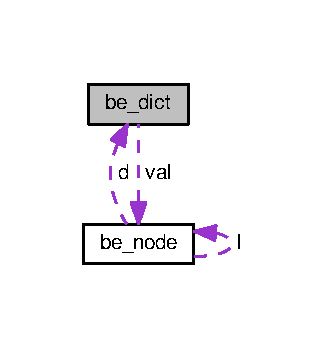
\includegraphics[width=157pt]{structbe__dict__coll__graph}
\end{center}
\end{figure}
\subsection*{Public Attributes}
\begin{DoxyCompactItemize}
\item 
\mbox{\Hypertarget{structbe__dict_a6ae73ce3648305247414d7565172ce68}\label{structbe__dict_a6ae73ce3648305247414d7565172ce68}} 
char $\ast$ {\bfseries key}
\item 
\mbox{\Hypertarget{structbe__dict_ae6dea60cf197f99318e44410440ec6af}\label{structbe__dict_ae6dea60cf197f99318e44410440ec6af}} 
struct \hyperlink{structbe__node}{be\+\_\+node} $\ast$ {\bfseries val}
\end{DoxyCompactItemize}


The documentation for this struct was generated from the following file\+:\begin{DoxyCompactItemize}
\item 
lib/bencode.\+h\end{DoxyCompactItemize}

\hypertarget{structbe__node}{}\section{be\+\_\+node Struct Reference}
\label{structbe__node}\index{be\+\_\+node@{be\+\_\+node}}


Collaboration diagram for be\+\_\+node\+:\nopagebreak
\begin{figure}[H]
\begin{center}
\leavevmode
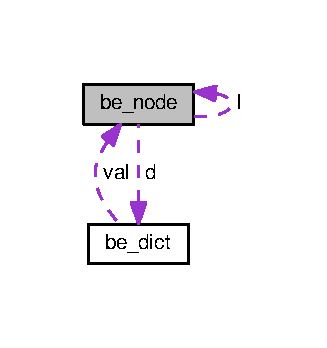
\includegraphics[width=157pt]{structbe__node__coll__graph}
\end{center}
\end{figure}
\subsection*{Public Attributes}
\begin{DoxyCompactItemize}
\item 
\mbox{\Hypertarget{structbe__node_a88d2500935e80562cd0ec9bf5a88ed45}\label{structbe__node_a88d2500935e80562cd0ec9bf5a88ed45}} 
be\+\_\+type {\bfseries type}
\item 
\mbox{\Hypertarget{structbe__node_af6e101f7301823d24fcda7a3e8be7e7d}\label{structbe__node_af6e101f7301823d24fcda7a3e8be7e7d}} 
\begin{tabbing}
xx\=xx\=xx\=xx\=xx\=xx\=xx\=xx\=xx\=\kill
union \{\\
\>char $\ast$ {\bfseries s}\\
\>long long {\bfseries i}\\
\>struct \hyperlink{structbe__node}{be\_node} $\ast$$\ast$ {\bfseries l}\\
\>struct \hyperlink{structbe__dict}{be\_dict} $\ast$ {\bfseries d}\\
\} {\bfseries val}\\

\end{tabbing}\end{DoxyCompactItemize}


The documentation for this struct was generated from the following file\+:\begin{DoxyCompactItemize}
\item 
lib/bencode.\+h\end{DoxyCompactItemize}

\hypertarget{structbInt}{}\section{b\+Int Struct Reference}
\label{structbInt}\index{b\+Int@{b\+Int}}
\subsection*{Public Attributes}
\begin{DoxyCompactItemize}
\item 
\mbox{\Hypertarget{structbInt_a2f9e3b9f6687d378cdab799d5eb5205c}\label{structbInt_a2f9e3b9f6687d378cdab799d5eb5205c}} 
uint8\+\_\+t {\bfseries i1}
\item 
\mbox{\Hypertarget{structbInt_aab28c4437083187b2374ba69e2353ece}\label{structbInt_aab28c4437083187b2374ba69e2353ece}} 
uint8\+\_\+t {\bfseries i2}
\item 
\mbox{\Hypertarget{structbInt_a3a44f29a66a9a97ac6b79d6fa53664ba}\label{structbInt_a3a44f29a66a9a97ac6b79d6fa53664ba}} 
uint8\+\_\+t {\bfseries i3}
\item 
\mbox{\Hypertarget{structbInt_afeeae065a1c51d70a1e8e34bdd4eba02}\label{structbInt_afeeae065a1c51d70a1e8e34bdd4eba02}} 
uint8\+\_\+t {\bfseries i4}
\end{DoxyCompactItemize}


The documentation for this struct was generated from the following file\+:\begin{DoxyCompactItemize}
\item 
lib/\hyperlink{peer_8h}{peer.\+h}\end{DoxyCompactItemize}

\hypertarget{structpwp_1_1client__state}{}\section{pwp\+:\+:client\+\_\+state Struct Reference}
\label{structpwp_1_1client__state}\index{pwp\+::client\+\_\+state@{pwp\+::client\+\_\+state}}
\subsection*{Public Attributes}
\begin{DoxyCompactItemize}
\item 
\mbox{\Hypertarget{structpwp_1_1client__state_a134704e7cdd2e26181fead2dffc795e1}\label{structpwp_1_1client__state_a134704e7cdd2e26181fead2dffc795e1}} 
bool {\bfseries am\+\_\+choking} = true
\item 
\mbox{\Hypertarget{structpwp_1_1client__state_a8376b624ad153316a0a7317f99da97c2}\label{structpwp_1_1client__state_a8376b624ad153316a0a7317f99da97c2}} 
bool {\bfseries am\+\_\+interested} = true
\end{DoxyCompactItemize}


The documentation for this struct was generated from the following file\+:\begin{DoxyCompactItemize}
\item 
lib/\hyperlink{peer_8h}{peer.\+h}\end{DoxyCompactItemize}

\hypertarget{structt__udp_1_1connect__request}{}\section{t\+\_\+udp\+:\+:connect\+\_\+request Struct Reference}
\label{structt__udp_1_1connect__request}\index{t\+\_\+udp\+::connect\+\_\+request@{t\+\_\+udp\+::connect\+\_\+request}}
\subsection*{Public Attributes}
\begin{DoxyCompactItemize}
\item 
int64\+\_\+t \hyperlink{structt__udp_1_1connect__request_a74e7bf8d757ea8c891cbd7abeeb07baa}{protocol\+\_\+id} = 0x41727101980
\item 
int32\+\_\+t \hyperlink{structt__udp_1_1connect__request_ae7598b55825c7ee92c38f1a35e36ba31}{action} = 0
\item 
\mbox{\Hypertarget{structt__udp_1_1connect__request_a3b32bfc52d06edcf986cb00a7ce60b17}\label{structt__udp_1_1connect__request_a3b32bfc52d06edcf986cb00a7ce60b17}} 
int32\+\_\+t {\bfseries transaction\+\_\+id}
\end{DoxyCompactItemize}


\subsection{Member Data Documentation}
\mbox{\Hypertarget{structt__udp_1_1connect__request_ae7598b55825c7ee92c38f1a35e36ba31}\label{structt__udp_1_1connect__request_ae7598b55825c7ee92c38f1a35e36ba31}} 
\index{t\+\_\+udp\+::connect\+\_\+request@{t\+\_\+udp\+::connect\+\_\+request}!action@{action}}
\index{action@{action}!t\+\_\+udp\+::connect\+\_\+request@{t\+\_\+udp\+::connect\+\_\+request}}
\subsubsection{\texorpdfstring{action}{action}}
{\footnotesize\ttfamily int32\+\_\+t t\+\_\+udp\+::connect\+\_\+request\+::action = 0}

Connection Value \mbox{\Hypertarget{structt__udp_1_1connect__request_a74e7bf8d757ea8c891cbd7abeeb07baa}\label{structt__udp_1_1connect__request_a74e7bf8d757ea8c891cbd7abeeb07baa}} 
\index{t\+\_\+udp\+::connect\+\_\+request@{t\+\_\+udp\+::connect\+\_\+request}!protocol\+\_\+id@{protocol\+\_\+id}}
\index{protocol\+\_\+id@{protocol\+\_\+id}!t\+\_\+udp\+::connect\+\_\+request@{t\+\_\+udp\+::connect\+\_\+request}}
\subsubsection{\texorpdfstring{protocol\+\_\+id}{protocol\_id}}
{\footnotesize\ttfamily int64\+\_\+t t\+\_\+udp\+::connect\+\_\+request\+::protocol\+\_\+id = 0x41727101980}

Magic Constant 

The documentation for this struct was generated from the following file\+:\begin{DoxyCompactItemize}
\item 
lib/\hyperlink{tracker__udp_8hpp}{tracker\+\_\+udp.\+hpp}\end{DoxyCompactItemize}

\hypertarget{structt__udp_1_1connect__response}{}\section{t\+\_\+udp\+:\+:connect\+\_\+response Struct Reference}
\label{structt__udp_1_1connect__response}\index{t\+\_\+udp\+::connect\+\_\+response@{t\+\_\+udp\+::connect\+\_\+response}}
\subsection*{Public Attributes}
\begin{DoxyCompactItemize}
\item 
int32\+\_\+t \hyperlink{structt__udp_1_1connect__response_a72371c40b24c52782ef0d03ca61c57e3}{action} = 0
\item 
\mbox{\Hypertarget{structt__udp_1_1connect__response_af5f97e3b41bd74d238f78a2233bd53d5}\label{structt__udp_1_1connect__response_af5f97e3b41bd74d238f78a2233bd53d5}} 
int32\+\_\+t {\bfseries transaction\+\_\+id}
\item 
\mbox{\Hypertarget{structt__udp_1_1connect__response_aa9e3aec7f9a33e92c59bcf548a1d83af}\label{structt__udp_1_1connect__response_aa9e3aec7f9a33e92c59bcf548a1d83af}} 
int64\+\_\+t {\bfseries connection\+\_\+id}
\end{DoxyCompactItemize}


\subsection{Member Data Documentation}
\mbox{\Hypertarget{structt__udp_1_1connect__response_a72371c40b24c52782ef0d03ca61c57e3}\label{structt__udp_1_1connect__response_a72371c40b24c52782ef0d03ca61c57e3}} 
\index{t\+\_\+udp\+::connect\+\_\+response@{t\+\_\+udp\+::connect\+\_\+response}!action@{action}}
\index{action@{action}!t\+\_\+udp\+::connect\+\_\+response@{t\+\_\+udp\+::connect\+\_\+response}}
\subsubsection{\texorpdfstring{action}{action}}
{\footnotesize\ttfamily int32\+\_\+t t\+\_\+udp\+::connect\+\_\+response\+::action = 0}

Connection Value 

The documentation for this struct was generated from the following file\+:\begin{DoxyCompactItemize}
\item 
lib/\hyperlink{tracker__udp_8hpp}{tracker\+\_\+udp.\+hpp}\end{DoxyCompactItemize}

\hypertarget{structpwp_1_1peer}{}\section{pwp\+:\+:peer Struct Reference}
\label{structpwp_1_1peer}\index{pwp\+::peer@{pwp\+::peer}}
\subsection*{Public Member Functions}
\begin{DoxyCompactItemize}
\item 
\mbox{\Hypertarget{structpwp_1_1peer_a63214c33b38e8ac1b1b8a23f724a0682}\label{structpwp_1_1peer_a63214c33b38e8ac1b1b8a23f724a0682}} 
bool {\bfseries operator==} (\hyperlink{structpwp_1_1peer}{peer} const \&rhs) const
\item 
\mbox{\Hypertarget{structpwp_1_1peer_a41fbc7e5f9d84a47224c61bd2b5ca9a3}\label{structpwp_1_1peer_a41fbc7e5f9d84a47224c61bd2b5ca9a3}} 
bool {\bfseries operator$>$} (\hyperlink{structpwp_1_1peer}{peer} const \&rhs) const
\end{DoxyCompactItemize}
\subsection*{Public Attributes}
\begin{DoxyCompactItemize}
\item 
ip\+::address \hyperlink{structpwp_1_1peer_a862dc1b14fd2e8485cc4c080bbe74e99}{addr}
\item 
\mbox{\Hypertarget{structpwp_1_1peer_accc9b1eb439425e9b944ed6ca966c8a4}\label{structpwp_1_1peer_accc9b1eb439425e9b944ed6ca966c8a4}} 
uint {\bfseries port}
\item 
std\+::string \hyperlink{structpwp_1_1peer_a93c9dfe3e8766d364887f615d0880777}{peer\+\_\+id}
\end{DoxyCompactItemize}


\subsection{Member Data Documentation}
\mbox{\Hypertarget{structpwp_1_1peer_a862dc1b14fd2e8485cc4c080bbe74e99}\label{structpwp_1_1peer_a862dc1b14fd2e8485cc4c080bbe74e99}} 
\index{pwp\+::peer@{pwp\+::peer}!addr@{addr}}
\index{addr@{addr}!pwp\+::peer@{pwp\+::peer}}
\subsubsection{\texorpdfstring{addr}{addr}}
{\footnotesize\ttfamily ip\+::address pwp\+::peer\+::addr}

\hyperlink{classPeer}{Peer}\textquotesingle{}s IP address (both v4 and v6) \mbox{\Hypertarget{structpwp_1_1peer_a93c9dfe3e8766d364887f615d0880777}\label{structpwp_1_1peer_a93c9dfe3e8766d364887f615d0880777}} 
\index{pwp\+::peer@{pwp\+::peer}!peer\+\_\+id@{peer\+\_\+id}}
\index{peer\+\_\+id@{peer\+\_\+id}!pwp\+::peer@{pwp\+::peer}}
\subsubsection{\texorpdfstring{peer\+\_\+id}{peer\_id}}
{\footnotesize\ttfamily std\+::string pwp\+::peer\+::peer\+\_\+id}

20 bytes peer id string 

The documentation for this struct was generated from the following file\+:\begin{DoxyCompactItemize}
\item 
lib/\hyperlink{peer_8h}{peer.\+h}\end{DoxyCompactItemize}

\hypertarget{classPeer}{}\section{Peer Class Reference}
\label{classPeer}\index{Peer@{Peer}}


The documentation for this class was generated from the following file\+:\begin{DoxyCompactItemize}
\item 
lib/peer.\+hpp\end{DoxyCompactItemize}

\hypertarget{structpwp_1_1peer__connection}{}\section{pwp\+:\+:peer\+\_\+connection Struct Reference}
\label{structpwp_1_1peer__connection}\index{pwp\+::peer\+\_\+connection@{pwp\+::peer\+\_\+connection}}


Collaboration diagram for pwp\+:\+:peer\+\_\+connection\+:\nopagebreak
\begin{figure}[H]
\begin{center}
\leavevmode
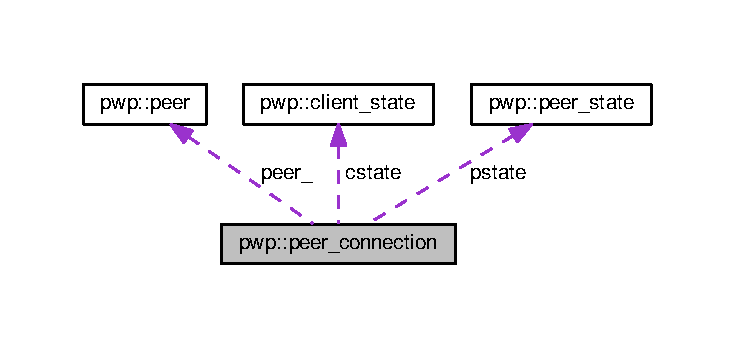
\includegraphics[width=350pt]{structpwp_1_1peer__connection__coll__graph}
\end{center}
\end{figure}
\subsection*{Public Attributes}
\begin{DoxyCompactItemize}
\item 
\mbox{\Hypertarget{structpwp_1_1peer__connection_a467a52a32ff0250d977b69026edce52c}\label{structpwp_1_1peer__connection_a467a52a32ff0250d977b69026edce52c}} 
struct \hyperlink{structpwp_1_1peer}{peer} {\bfseries peer\+\_\+}
\item 
\mbox{\Hypertarget{structpwp_1_1peer__connection_a7760fde637e5b09ba43010b8e5b4cdf0}\label{structpwp_1_1peer__connection_a7760fde637e5b09ba43010b8e5b4cdf0}} 
\hyperlink{structpwp_1_1client__state}{client\+\_\+state} {\bfseries cstate}
\item 
\mbox{\Hypertarget{structpwp_1_1peer__connection_a6720cb5711a2f21d8025e45a9de05a85}\label{structpwp_1_1peer__connection_a6720cb5711a2f21d8025e45a9de05a85}} 
\hyperlink{structpwp_1_1peer__state}{peer\+\_\+state} {\bfseries pstate}
\item 
\mbox{\Hypertarget{structpwp_1_1peer__connection_a61d97fcac3bd21d477a1204a3803a639}\label{structpwp_1_1peer__connection_a61d97fcac3bd21d477a1204a3803a639}} 
boost\+::dynamic\+\_\+bitset {\bfseries bitfield}
\item 
\mbox{\Hypertarget{structpwp_1_1peer__connection_a20b428bd7fb2d3de54016c8801cb98b8}\label{structpwp_1_1peer__connection_a20b428bd7fb2d3de54016c8801cb98b8}} 
std\+::shared\+\_\+ptr$<$ boost\+::asio\+::ip\+::tcp\+::socket $>$ {\bfseries socket}
\end{DoxyCompactItemize}


The documentation for this struct was generated from the following file\+:\begin{DoxyCompactItemize}
\item 
lib/\hyperlink{peer_8h}{peer.\+h}\end{DoxyCompactItemize}

\hypertarget{structpwp_1_1peer__state}{}\section{pwp\+:\+:peer\+\_\+state Struct Reference}
\label{structpwp_1_1peer__state}\index{pwp\+::peer\+\_\+state@{pwp\+::peer\+\_\+state}}
\subsection*{Public Attributes}
\begin{DoxyCompactItemize}
\item 
\mbox{\Hypertarget{structpwp_1_1peer__state_ab98eeb7525aa57db451b4b7446f47ba3}\label{structpwp_1_1peer__state_ab98eeb7525aa57db451b4b7446f47ba3}} 
bool {\bfseries peer\+\_\+choking} = true
\item 
\mbox{\Hypertarget{structpwp_1_1peer__state_a3d6e90c271ea2c48b3dbada7371e4757}\label{structpwp_1_1peer__state_a3d6e90c271ea2c48b3dbada7371e4757}} 
bool {\bfseries peer\+\_\+interested} = false
\end{DoxyCompactItemize}


The documentation for this struct was generated from the following file\+:\begin{DoxyCompactItemize}
\item 
lib/\hyperlink{peer_8h}{peer.\+h}\end{DoxyCompactItemize}

\hypertarget{structRequestMsg}{}\section{Request\+Msg Struct Reference}
\label{structRequestMsg}\index{Request\+Msg@{Request\+Msg}}
\subsection*{Public Attributes}
\begin{DoxyCompactItemize}
\item 
\mbox{\Hypertarget{structRequestMsg_a7f20219554383b1ed60aed8acec7a287}\label{structRequestMsg_a7f20219554383b1ed60aed8acec7a287}} 
size\+\_\+t {\bfseries index}
\item 
\mbox{\Hypertarget{structRequestMsg_a6197b604a388f266a963c3011114092c}\label{structRequestMsg_a6197b604a388f266a963c3011114092c}} 
size\+\_\+t {\bfseries begin}
\item 
\mbox{\Hypertarget{structRequestMsg_a764a4087dfa01afbf2eaedd31c4695f1}\label{structRequestMsg_a764a4087dfa01afbf2eaedd31c4695f1}} 
size\+\_\+t {\bfseries length}
\end{DoxyCompactItemize}


The documentation for this struct was generated from the following file\+:\begin{DoxyCompactItemize}
\item 
lib/filehandler.\+hpp\end{DoxyCompactItemize}

\hypertarget{structTorrent}{}\section{Torrent Struct Reference}
\label{structTorrent}\index{Torrent@{Torrent}}


Struct to store all the information of a torrent.  




{\ttfamily \#include $<$torrentparser.\+hpp$>$}

\subsection*{Public Attributes}
\begin{DoxyCompactItemize}
\item 
\mbox{\Hypertarget{structTorrent_a634e08dc5c95e76117074acb5f633a90}\label{structTorrent_a634e08dc5c95e76117074acb5f633a90}} 
std\+::vector$<$ std\+::string $>$ {\bfseries trackers}
\item 
\mbox{\Hypertarget{structTorrent_af0f3f1ae144a53edfd6f526abe35911a}\label{structTorrent_af0f3f1ae144a53edfd6f526abe35911a}} 
std\+::string {\bfseries name}
\item 
\mbox{\Hypertarget{structTorrent_af35506b5ff7dfa2479dfafa5db46ccb7}\label{structTorrent_af35506b5ff7dfa2479dfafa5db46ccb7}} 
int {\bfseries piece\+\_\+length}
\item 
\mbox{\Hypertarget{structTorrent_adf5e9b81258493066f0649348fec1383}\label{structTorrent_adf5e9b81258493066f0649348fec1383}} 
std\+::string {\bfseries pieces}
\item 
\mbox{\Hypertarget{structTorrent_a3f559e759bb388621ed3ca287e0dce4b}\label{structTorrent_a3f559e759bb388621ed3ca287e0dce4b}} 
size\+\_\+t {\bfseries num\+\_\+pieces}
\item 
\mbox{\Hypertarget{structTorrent_a3cf53601cc00765215995fc7f093e5cd}\label{structTorrent_a3cf53601cc00765215995fc7f093e5cd}} 
std\+::vector$<$ \hyperlink{structTorrentFile}{Torrent\+File} $>$ {\bfseries files}
\item 
\mbox{\Hypertarget{structTorrent_a8c811cd46d8935b7c25f00c9819463c2}\label{structTorrent_a8c811cd46d8935b7c25f00c9819463c2}} 
boost\+::dynamic\+\_\+bitset {\bfseries bitfield}
\item 
\mbox{\Hypertarget{structTorrent_a9745fb134056ea76dc14cdbd11b58f3e}\label{structTorrent_a9745fb134056ea76dc14cdbd11b58f3e}} 
bool {\bfseries is\+\_\+single} = false
\end{DoxyCompactItemize}


\subsection{Detailed Description}
Struct to store all the information of a torrent. 

The documentation for this struct was generated from the following file\+:\begin{DoxyCompactItemize}
\item 
lib/\hyperlink{torrentparser_8hpp}{torrentparser.\+hpp}\end{DoxyCompactItemize}

\hypertarget{structTorrentFile}{}\section{Torrent\+File Struct Reference}
\label{structTorrentFile}\index{Torrent\+File@{Torrent\+File}}
\subsection*{Public Attributes}
\begin{DoxyCompactItemize}
\item 
\mbox{\Hypertarget{structTorrentFile_af01926bfbda73df36e9648d35c973470}\label{structTorrentFile_af01926bfbda73df36e9648d35c973470}} 
std\+::vector$<$ std\+::string $>$ {\bfseries path}
\item 
\mbox{\Hypertarget{structTorrentFile_a325e8999959721baf05d23b14349dcd7}\label{structTorrentFile_a325e8999959721baf05d23b14349dcd7}} 
long int {\bfseries length}
\end{DoxyCompactItemize}


The documentation for this struct was generated from the following file\+:\begin{DoxyCompactItemize}
\item 
lib/torrentparser.\+hpp\end{DoxyCompactItemize}

\hypertarget{structtracker_1_1TParameter}{}\section{tracker\+:\+:T\+Parameter Struct Reference}
\label{structtracker_1_1TParameter}\index{tracker\+::\+T\+Parameter@{tracker\+::\+T\+Parameter}}
\subsection*{Public Attributes}
\begin{DoxyCompactItemize}
\item 
\mbox{\Hypertarget{structtracker_1_1TParameter_aefb0050bfd99eb6a30b547b3e8891dcd}\label{structtracker_1_1TParameter_aefb0050bfd99eb6a30b547b3e8891dcd}} 
string {\bfseries info\+\_\+hash}
\item 
\mbox{\Hypertarget{structtracker_1_1TParameter_aa4fecf8ffb04fac7e3929cef30f032ac}\label{structtracker_1_1TParameter_aa4fecf8ffb04fac7e3929cef30f032ac}} 
string {\bfseries peer\+\_\+id}
\item 
\mbox{\Hypertarget{structtracker_1_1TParameter_a37c80391b4706f15068938a5186ebcb5}\label{structtracker_1_1TParameter_a37c80391b4706f15068938a5186ebcb5}} 
uint {\bfseries port}
\item 
\mbox{\Hypertarget{structtracker_1_1TParameter_aca491cdfef7ea15eb10768389dd8d043}\label{structtracker_1_1TParameter_aca491cdfef7ea15eb10768389dd8d043}} 
uint {\bfseries uploaded}
\item 
\mbox{\Hypertarget{structtracker_1_1TParameter_a4e7ad869a2a84c1773fa97e2f8ac7a70}\label{structtracker_1_1TParameter_a4e7ad869a2a84c1773fa97e2f8ac7a70}} 
uint {\bfseries downloaded}
\item 
\mbox{\Hypertarget{structtracker_1_1TParameter_ac4cfc3ad1c6e7cf4301d1940723e331a}\label{structtracker_1_1TParameter_ac4cfc3ad1c6e7cf4301d1940723e331a}} 
uint {\bfseries left}
\item 
\mbox{\Hypertarget{structtracker_1_1TParameter_aa20b3bfd0be9058a717e277e917a1604}\label{structtracker_1_1TParameter_aa20b3bfd0be9058a717e277e917a1604}} 
bool {\bfseries compact}
\item 
\mbox{\Hypertarget{structtracker_1_1TParameter_a21bb71f791e005b04f27d2d1ea1b7907}\label{structtracker_1_1TParameter_a21bb71f791e005b04f27d2d1ea1b7907}} 
uint16\+\_\+t {\bfseries numwant}
\item 
\mbox{\Hypertarget{structtracker_1_1TParameter_a54bbbc985f11ea3d022d24e2dd9d8a92}\label{structtracker_1_1TParameter_a54bbbc985f11ea3d022d24e2dd9d8a92}} 
string {\bfseries key}
\item 
\mbox{\Hypertarget{structtracker_1_1TParameter_ae88632924fe55b815994a2dc2bce67a2}\label{structtracker_1_1TParameter_ae88632924fe55b815994a2dc2bce67a2}} 
char $\ast$ {\bfseries info\+\_\+hash\+\_\+raw}
\end{DoxyCompactItemize}


The documentation for this struct was generated from the following file\+:\begin{DoxyCompactItemize}
\item 
lib/tracker.\+h\end{DoxyCompactItemize}

\chapter{File Documentation}
\hypertarget{peer_8h}{}\section{lib/peer.h File Reference}
\label{peer_8h}\index{lib/peer.\+h@{lib/peer.\+h}}
{\ttfamily \#include $<$string$>$}\newline
{\ttfamily \#include $<$memory$>$}\newline
{\ttfamily \#include $<$vector$>$}\newline
{\ttfamily \#include $<$boost/asio.\+hpp$>$}\newline
{\ttfamily \#include $<$boost/array.\+hpp$>$}\newline
{\ttfamily \#include $<$boost/chrono.\+hpp$>$}\newline
{\ttfamily \#include $<$boost/dynamic\+\_\+bitset.\+hpp$>$}\newline
{\ttfamily \#include $<$boost/thread.\+hpp$>$}\newline
{\ttfamily \#include \char`\"{}torrentparser.\+hpp\char`\"{}}\newline
Include dependency graph for peer.\+h\+:\nopagebreak
\begin{figure}[H]
\begin{center}
\leavevmode
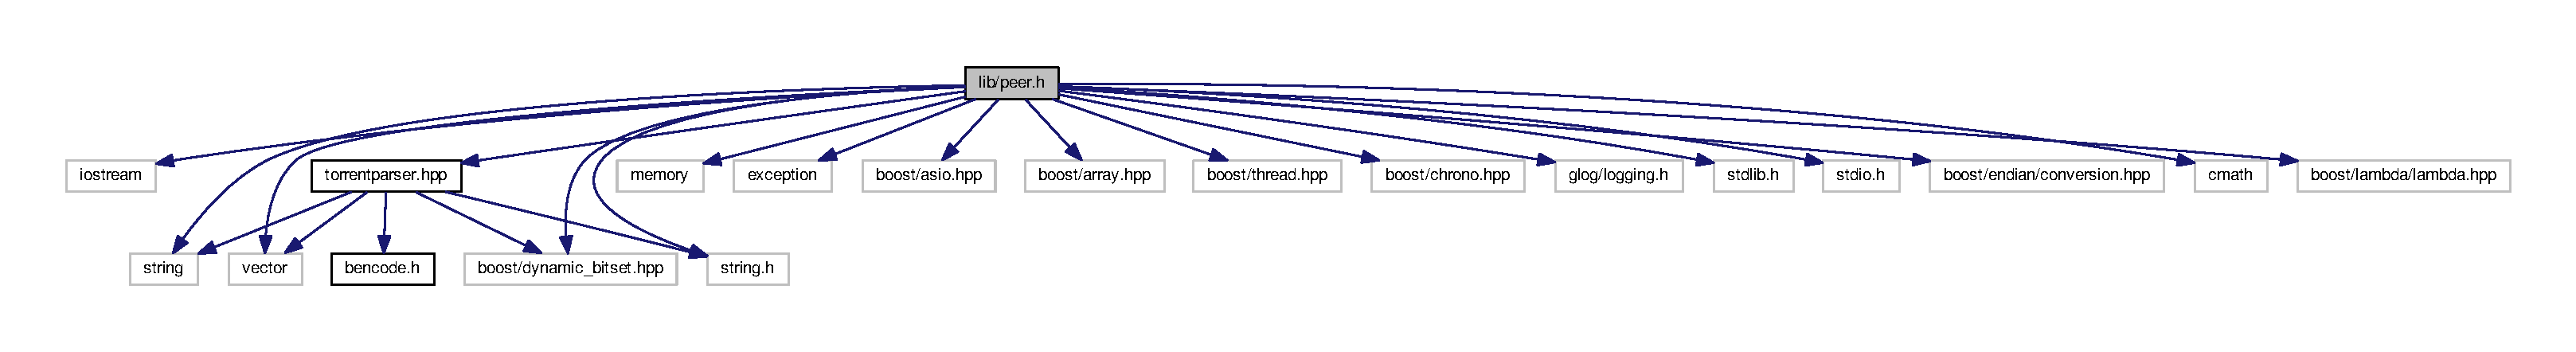
\includegraphics[width=350pt]{peer_8h__incl}
\end{center}
\end{figure}
This graph shows which files directly or indirectly include this file\+:\nopagebreak
\begin{figure}[H]
\begin{center}
\leavevmode
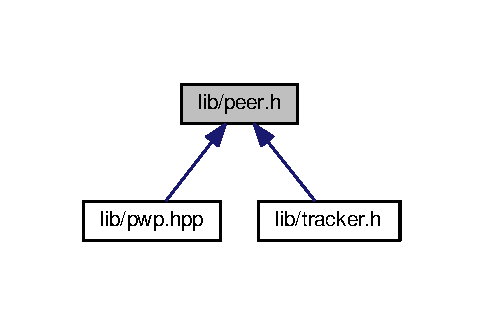
\includegraphics[width=232pt]{peer_8h__dep__incl}
\end{center}
\end{figure}
\subsection*{Classes}
\begin{DoxyCompactItemize}
\item 
struct \hyperlink{structpwp_1_1client__state}{pwp\+::client\+\_\+state}
\item 
struct \hyperlink{structpwp_1_1peer__state}{pwp\+::peer\+\_\+state}
\item 
struct \hyperlink{structpwp_1_1peer}{pwp\+::peer}
\item 
struct \hyperlink{structpwp_1_1peer__connection}{pwp\+::peer\+\_\+connection}
\item 
struct \hyperlink{structbInt}{b\+Int}
\end{DoxyCompactItemize}
\subsection*{Namespaces}
\begin{DoxyCompactItemize}
\item 
 \hyperlink{namespacepwp}{pwp}
\end{DoxyCompactItemize}
\subsection*{Macros}
\begin{DoxyCompactItemize}
\item 
\mbox{\Hypertarget{peer_8h_ac4f8a5810b63e63e2f2fe4642025530f}\label{peer_8h_ac4f8a5810b63e63e2f2fe4642025530f}} 
\#define {\bfseries D\+E\+F\+A\+U\+L\+T\+\_\+\+B\+U\+F\+F\+\_\+\+S\+I\+ZE}~128
\end{DoxyCompactItemize}
\subsection*{Typedefs}
\begin{DoxyCompactItemize}
\item 
typedef std\+::shared\+\_\+ptr$<$ std\+::vector$<$ \hyperlink{structpwp_1_1peer}{pwp\+::peer} $>$ $>$ \hyperlink{namespacepwp_ad07fa6df116b205302ad5ec172277184}{pwp\+::\+Peer\+List}
\item 
\mbox{\Hypertarget{namespacepwp_a174e8f020062fa10258b0d28f00d79ff}\label{namespacepwp_a174e8f020062fa10258b0d28f00d79ff}} 
typedef std\+::shared\+\_\+ptr$<$ std\+::vector$<$ \hyperlink{structpwp_1_1peer__connection}{pwp\+::peer\+\_\+connection} $>$ $>$ {\bfseries pwp\+::\+Peer\+Connected}
\item 
\mbox{\Hypertarget{peer_8h_ad61558c1c2cfe845f0a80296761f4652}\label{peer_8h_ad61558c1c2cfe845f0a80296761f4652}} 
typedef struct \hyperlink{structbInt}{b\+Int} {\bfseries b\+Int}
\end{DoxyCompactItemize}
\subsection*{Functions}
\begin{DoxyCompactItemize}
\item 
\mbox{\Hypertarget{peer_8h_ab03bdb6193d51579d2e14c3fdf704b6d}\label{peer_8h_ab03bdb6193d51579d2e14c3fdf704b6d}} 
void {\bfseries add\+\_\+active\+\_\+peer} ()
\item 
\mbox{\Hypertarget{peer_8h_a536da2a1a4821536d1ae07a26a96e60a}\label{peer_8h_a536da2a1a4821536d1ae07a26a96e60a}} 
void {\bfseries rm\+\_\+active\+\_\+peer} ()
\item 
\mbox{\Hypertarget{namespacepwp_ab82c0d015f6ba23e766c4b942a125b5f}\label{namespacepwp_ab82c0d015f6ba23e766c4b942a125b5f}} 
void {\bfseries pwp\+::manage\+\_\+peer\+\_\+connection} (\hyperlink{namespacepwp_ad07fa6df116b205302ad5ec172277184}{pwp\+::\+Peer\+List} peer\+\_\+list, char $\ast$info\+\_\+hash)
\item 
\mbox{\Hypertarget{namespacepwp_a5f03cde749af88a393c999545830b192}\label{namespacepwp_a5f03cde749af88a393c999545830b192}} 
void {\bfseries pwp\+::get\+\_\+peer\+\_\+id} (std\+::string $\ast$id)
\item 
void \hyperlink{namespacepwp_a6062876f4d4d4d6ee19341a79a797864}{pwp\+::build\+\_\+handshake} (char $\ast$info\+\_\+hash, std\+::vector$<$ uint8\+\_\+t $>$ \&handshake)
\item 
int \hyperlink{namespacepwp_a851ddc0e8fb2eb0a86317cc944c4a927}{pwp\+::send\+\_\+handshake} (\hyperlink{structpwp_1_1peer__connection}{pwp\+::peer\+\_\+connection} \&peerc\+\_\+t, const std\+::vector$<$ uint8\+\_\+t $>$ handshake, std\+::vector$<$ uint8\+\_\+t $>$ \&response)
\item 
\mbox{\Hypertarget{namespacepwp_ae2eeca61e271fabff5fa45308396009e}\label{namespacepwp_ae2eeca61e271fabff5fa45308396009e}} 
void {\bfseries pwp\+::handshake\+\_\+request\+\_\+manager} (const std\+::array$<$ char, 256 $>$ \&handshake, const \hyperlink{structpwp_1_1peer}{pwp\+::peer} t\+\_\+peer, const char $\ast$info\+\_\+hash, pwp\+::\+Peer\+Connected valid\+\_\+peer)
\item 
\mbox{\Hypertarget{namespacepwp_aed118903b8345e62507ade49c6032d32}\label{namespacepwp_aed118903b8345e62507ade49c6032d32}} 
int {\bfseries pwp\+::verify\+\_\+handshake} (const std\+::vector$<$ uint8\+\_\+t $>$ handshake, size\+\_\+t len, const \hyperlink{structpwp_1_1peer}{pwp\+::peer} t\+\_\+peer, const char $\ast$info\+\_\+hash)
\item 
void \hyperlink{namespacepwp_ae8331eb5e3c98deddc6022dad92352f6}{pwp\+::remove\+\_\+invalid\+\_\+peer} (\hyperlink{namespacepwp_ad07fa6df116b205302ad5ec172277184}{pwp\+::\+Peer\+List} peer\+\_\+list)
\begin{DoxyCompactList}\small\item\em Find invalid peers and remove it. \end{DoxyCompactList}\item 
void \hyperlink{namespacepwp_a62060bdcdc80541b0892e26fbeab1e91}{pwp\+::pwp\+\_\+protocol\+\_\+manager} (\hyperlink{structpwp_1_1peer}{pwp\+::peer} peer\+\_\+, const std\+::vector$<$ uint8\+\_\+t $>$ \&handshake, const char $\ast$info\+\_\+hash, \hyperlink{structtorr_1_1Torrent}{Torrent} \&torrent)
\begin{DoxyCompactList}\small\item\em Manager of the entire P\+WP protocol. \end{DoxyCompactList}\item 
\mbox{\Hypertarget{peer_8h_a271dd525a536a4182946e975569203bd}\label{peer_8h_a271dd525a536a4182946e975569203bd}} 
uint32\+\_\+t {\bfseries make\+\_\+int} (\hyperlink{structbInt}{b\+Int} bint)
\item 
\mbox{\Hypertarget{peer_8h_ac8b17972b6cc91299003983c8699ea0e}\label{peer_8h_ac8b17972b6cc91299003983c8699ea0e}} 
uint32\+\_\+t {\bfseries make\+\_\+int} (std\+::vector$<$ uint8\+\_\+t $>$ v)
\item 
\mbox{\Hypertarget{peer_8h_aa53a54b161cc4fd1306d84759a358067}\label{peer_8h_aa53a54b161cc4fd1306d84759a358067}} 
std\+::vector$<$ uint8\+\_\+t $>$ {\bfseries from\+\_\+int\+\_\+to\+\_\+bint} (uint integer)
\item 
\mbox{\Hypertarget{peer_8h_ab5548d1ece514e6fb8ccc19528b39904}\label{peer_8h_ab5548d1ece514e6fb8ccc19528b39904}} 
std\+::vector$<$ uint8\+\_\+t $>$ {\bfseries from\+\_\+int64\+\_\+to\+\_\+bint} (uint64\+\_\+t integer)
\item 
std\+::string \hyperlink{peer_8h_a9a16c464cd63530a7fbd80134c32f264}{string\+\_\+to\+\_\+hex} (const std\+::vector$<$ uint8\+\_\+t $>$ \&input)
\end{DoxyCompactItemize}
\subsection*{Variables}
\begin{DoxyCompactItemize}
\item 
boost\+::asio\+::io\+\_\+service \hyperlink{peer_8h_a7efe93eb3d4e0f0c9ab96fa5ae443fcd}{\+\_\+io\+\_\+service}
\item 
\mbox{\Hypertarget{peer_8h_afd3bb609482f388199b44f364c870321}\label{peer_8h_afd3bb609482f388199b44f364c870321}} 
int {\bfseries active\+\_\+peer}
\item 
boost\+::mutex \hyperlink{peer_8h_a821fac971970c19e5d4f57dd0486f019}{mtx\+\_\+peer\+\_\+num}
\end{DoxyCompactItemize}


\subsection{Detailed Description}
Peer\textquotesingle{}s data and P\+WP protocol interface

This define the basic P\+WP protocol structure along with peer interface 

\subsection{Function Documentation}
\mbox{\Hypertarget{peer_8h_a9a16c464cd63530a7fbd80134c32f264}\label{peer_8h_a9a16c464cd63530a7fbd80134c32f264}} 
\index{peer.\+h@{peer.\+h}!string\+\_\+to\+\_\+hex@{string\+\_\+to\+\_\+hex}}
\index{string\+\_\+to\+\_\+hex@{string\+\_\+to\+\_\+hex}!peer.\+h@{peer.\+h}}
\subsubsection{\texorpdfstring{string\+\_\+to\+\_\+hex()}{string\_to\_hex()}}
{\footnotesize\ttfamily std\+::string string\+\_\+to\+\_\+hex (\begin{DoxyParamCaption}\item[{const std\+::vector$<$ uint8\+\_\+t $>$ \&}]{input }\end{DoxyParamCaption})}

Takes vector of bytes and print its H\+EX rappresentation


\begin{DoxyParams}{Parameters}
{\em input} & The bytes to convert \\
\hline
\end{DoxyParams}
\begin{DoxyReturn}{Returns}
An H\+EX string
\end{DoxyReturn}
T\+O\+DO rename this nonsense function name 

\subsection{Variable Documentation}
\mbox{\Hypertarget{peer_8h_a7efe93eb3d4e0f0c9ab96fa5ae443fcd}\label{peer_8h_a7efe93eb3d4e0f0c9ab96fa5ae443fcd}} 
\index{peer.\+h@{peer.\+h}!\+\_\+io\+\_\+service@{\+\_\+io\+\_\+service}}
\index{\+\_\+io\+\_\+service@{\+\_\+io\+\_\+service}!peer.\+h@{peer.\+h}}
\subsubsection{\texorpdfstring{\+\_\+io\+\_\+service}{\_io\_service}}
{\footnotesize\ttfamily boost\+::asio\+::io\+\_\+service \+\_\+io\+\_\+service}

Global I\+O-\/\+Service \mbox{\Hypertarget{peer_8h_a821fac971970c19e5d4f57dd0486f019}\label{peer_8h_a821fac971970c19e5d4f57dd0486f019}} 
\index{peer.\+h@{peer.\+h}!mtx\+\_\+peer\+\_\+num@{mtx\+\_\+peer\+\_\+num}}
\index{mtx\+\_\+peer\+\_\+num@{mtx\+\_\+peer\+\_\+num}!peer.\+h@{peer.\+h}}
\subsubsection{\texorpdfstring{mtx\+\_\+peer\+\_\+num}{mtx\_peer\_num}}
{\footnotesize\ttfamily boost\+::mutex mtx\+\_\+peer\+\_\+num}

Mutex for the alive peers number 
\hypertarget{pwp_8hpp}{}\section{lib/pwp.hpp File Reference}
\label{pwp_8hpp}\index{lib/pwp.\+hpp@{lib/pwp.\+hpp}}
{\ttfamily \#include $<$iostream$>$}\newline
{\ttfamily \#include $<$boost/asio.\+hpp$>$}\newline
{\ttfamily \#include $<$boost/date\+\_\+time/posix\+\_\+time/posix\+\_\+time.\+hpp$>$}\newline
{\ttfamily \#include \char`\"{}torrentparser.\+hpp\char`\"{}}\newline
{\ttfamily \#include \char`\"{}peer.\+h\char`\"{}}\newline
Include dependency graph for pwp.\+hpp\+:\nopagebreak
\begin{figure}[H]
\begin{center}
\leavevmode
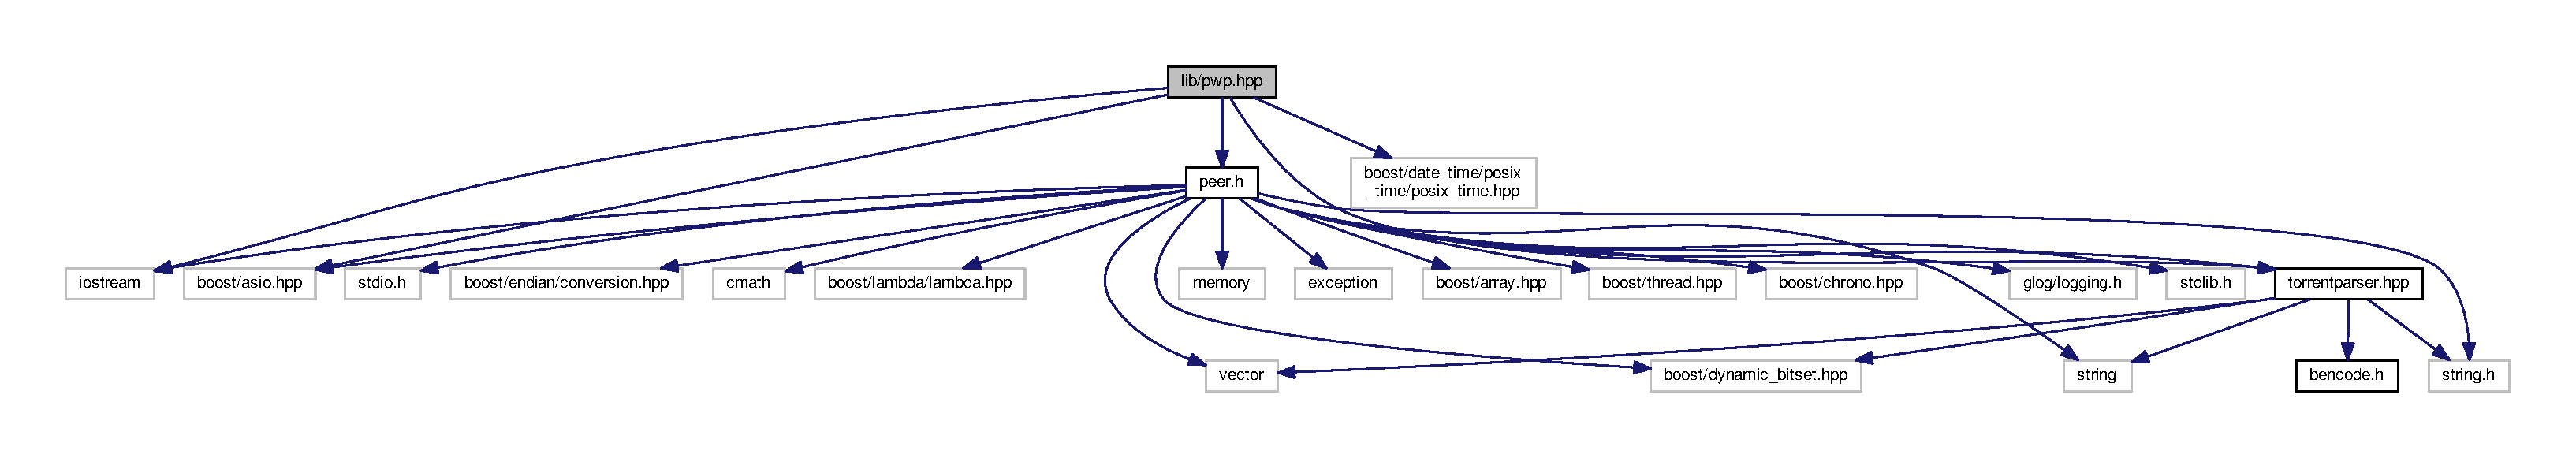
\includegraphics[width=350pt]{pwp_8hpp__incl}
\end{center}
\end{figure}
\subsection*{Namespaces}
\begin{DoxyCompactItemize}
\item 
 \hyperlink{namespacepwp__msg}{pwp\+\_\+msg}
\end{DoxyCompactItemize}
\subsection*{Macros}
\begin{DoxyCompactItemize}
\item 
\#define \hyperlink{pwp_8hpp_ada8ab189068d244326935c6e7926801f}{K\+E\+E\+P\+\_\+\+A\+L\+I\+V\+E\+\_\+\+T\+I\+ME}~75
\end{DoxyCompactItemize}
\subsection*{Enumerations}
\begin{DoxyCompactItemize}
\item 
enum \hyperlink{namespacepwp__msg_a0b9a29508f00a30e5138d2b78f4b1daf}{pwp\+\_\+msg\+::msg\+\_\+id} \{ \newline
\hyperlink{namespacepwp__msg_a0b9a29508f00a30e5138d2b78f4b1dafae1d8b3754d66ec7fcad827fb54eaeea2}{pwp\+\_\+msg\+::chocked} = 0x00, 
\hyperlink{namespacepwp__msg_a0b9a29508f00a30e5138d2b78f4b1dafa55689e288bf71e7737faaf385b1c528b}{pwp\+\_\+msg\+::unchocked} = 0x01, 
{\bfseries interested} = 0x02, 
{\bfseries not\+\_\+interested} = 0x03, 
\newline
{\bfseries have} = 0x04, 
\hyperlink{namespacepwp__msg_a0b9a29508f00a30e5138d2b78f4b1dafac3a2343a7b67a371e241ae2184bfe9cd}{pwp\+\_\+msg\+::bitfield} = 0x05, 
{\bfseries request} = 0x06, 
{\bfseries piece} = 0x07, 
\newline
{\bfseries cancel} = 0x08, 
{\bfseries port} = 0x09
 \}
\end{DoxyCompactItemize}
\subsection*{Functions}
\begin{DoxyCompactItemize}
\item 
bool \hyperlink{pwp_8hpp_a0bcf004164275de8518de37de3823f1c}{is\+\_\+inv\+\_\+address} (const boost\+::asio\+::ip\+::address \&addr)
\item 
void \hyperlink{namespacepwp__msg_a30c14bc06a8bb851ca79781cb9686b4f}{pwp\+\_\+msg\+::enable\+\_\+keep\+\_\+alive\+\_\+message} (\hyperlink{structpwp_1_1peer__connection}{pwp\+::peer\+\_\+connection} \&peer\+\_\+c)
\item 
int \hyperlink{namespacepwp__msg_aca807c6281879abef952f8feecccb6e8}{pwp\+\_\+msg\+::send\+\_\+msg} (\hyperlink{structpwp_1_1peer__connection}{pwp\+::peer\+\_\+connection} \&peer\+\_\+c, std\+::vector$<$ uint8\+\_\+t $>$ msg)
\begin{DoxyCompactList}\small\item\em Send {\ttfamily msg} to the peer specified in {\ttfamily peer\+\_\+c} \end{DoxyCompactList}\item 
\mbox{\Hypertarget{namespacepwp__msg_aa9cc2ccac70638ed59075f27f938b8ec}\label{namespacepwp__msg_aa9cc2ccac70638ed59075f27f938b8ec}} 
int {\bfseries pwp\+\_\+msg\+::get\+\_\+bitfield} (\hyperlink{structpwp_1_1peer__connection}{pwp\+::peer\+\_\+connection} \&peer\+\_\+c, \hyperlink{structTorrent}{Torrent} \&torrent)
\item 
\mbox{\Hypertarget{namespacepwp__msg_aec35de04a2f2d9cb6abdd777917cfaae}\label{namespacepwp__msg_aec35de04a2f2d9cb6abdd777917cfaae}} 
void {\bfseries pwp\+\_\+msg\+::read\+\_\+msg\+\_\+handler} (std\+::vector$<$ uint8\+\_\+t $>$ \&response, \hyperlink{structpwp_1_1peer__connection}{pwp\+::peer\+\_\+connection} \&peer\+\_\+c, \hyperlink{structTorrent}{Torrent} \&torrent, bool \&dead\+\_\+peer, boost\+::asio\+::deadline\+\_\+timer \&timer\+\_\+, const boost\+::system\+::error\+\_\+code \&error, size\+\_\+t bytes\+\_\+read)
\item 
\mbox{\Hypertarget{namespacepwp__msg_ab578b213d293636d33efc24382f16b25}\label{namespacepwp__msg_ab578b213d293636d33efc24382f16b25}} 
int {\bfseries pwp\+\_\+msg\+::sender} (\hyperlink{structpwp_1_1peer__connection}{pwp\+::peer\+\_\+connection} \&peer\+\_\+conn, \hyperlink{structTorrent}{Torrent} \&torrent, int \&old\+\_\+begin)
\end{DoxyCompactItemize}
\subsection*{Variables}
\begin{DoxyCompactItemize}
\item 
boost\+::asio\+::io\+\_\+service \hyperlink{pwp_8hpp_a7efe93eb3d4e0f0c9ab96fa5ae443fcd}{\+\_\+io\+\_\+service}
\item 
\mbox{\Hypertarget{pwp_8hpp_afd3bb609482f388199b44f364c870321}\label{pwp_8hpp_afd3bb609482f388199b44f364c870321}} 
int {\bfseries active\+\_\+peer}
\item 
\mbox{\Hypertarget{pwp_8hpp_a821fac971970c19e5d4f57dd0486f019}\label{pwp_8hpp_a821fac971970c19e5d4f57dd0486f019}} 
boost\+::mutex {\bfseries mtx\+\_\+peer\+\_\+num}
\item 
\mbox{\Hypertarget{namespacepwp__msg_ae962e65b1871714756b6aeb4722a8caf}\label{namespacepwp__msg_ae962e65b1871714756b6aeb4722a8caf}} 
enum \hyperlink{namespacepwp__msg_a0b9a29508f00a30e5138d2b78f4b1daf}{pwp\+\_\+msg\+::msg\+\_\+id} {\bfseries pwp\+\_\+msg\+::\+Peer\+List}
\item 
const std\+::vector$<$ uint8\+\_\+t $>$ \hyperlink{namespacepwp__msg_a695ee2efb59a7c258559f19440fe6998}{pwp\+\_\+msg\+::choke\+\_\+msg} = \{0,0,0,1,0\}
\item 
const std\+::vector$<$ uint8\+\_\+t $>$ \hyperlink{namespacepwp__msg_acdc5eb698534e84a15db0e061c511e7c}{pwp\+\_\+msg\+::unchoke\+\_\+msg} = \{0,0,0,1,1\}
\item 
const std\+::vector$<$ uint8\+\_\+t $>$ \hyperlink{namespacepwp__msg_afc68b17ce131c52fa0beb0cc7185778b}{pwp\+\_\+msg\+::interested\+\_\+msg} = \{0,0,0,1,2\}
\item 
const std\+::vector$<$ uint8\+\_\+t $>$ \hyperlink{namespacepwp__msg_a16a5f22f784d872342a82af9f6b77830}{pwp\+\_\+msg\+::non\+\_\+interested\+\_\+msg} = \{0,0,0,1,3\}
\end{DoxyCompactItemize}


\subsection{Detailed Description}
P\+WP protocol function

P\+WP protocol messagge specification and implementation 

\subsection{Macro Definition Documentation}
\mbox{\Hypertarget{pwp_8hpp_ada8ab189068d244326935c6e7926801f}\label{pwp_8hpp_ada8ab189068d244326935c6e7926801f}} 
\index{pwp.\+hpp@{pwp.\+hpp}!K\+E\+E\+P\+\_\+\+A\+L\+I\+V\+E\+\_\+\+T\+I\+ME@{K\+E\+E\+P\+\_\+\+A\+L\+I\+V\+E\+\_\+\+T\+I\+ME}}
\index{K\+E\+E\+P\+\_\+\+A\+L\+I\+V\+E\+\_\+\+T\+I\+ME@{K\+E\+E\+P\+\_\+\+A\+L\+I\+V\+E\+\_\+\+T\+I\+ME}!pwp.\+hpp@{pwp.\+hpp}}
\subsubsection{\texorpdfstring{K\+E\+E\+P\+\_\+\+A\+L\+I\+V\+E\+\_\+\+T\+I\+ME}{KEEP\_ALIVE\_TIME}}
{\footnotesize\ttfamily \#define K\+E\+E\+P\+\_\+\+A\+L\+I\+V\+E\+\_\+\+T\+I\+ME~75}

Default chocked message 

\subsection{Function Documentation}
\mbox{\Hypertarget{pwp_8hpp_a0bcf004164275de8518de37de3823f1c}\label{pwp_8hpp_a0bcf004164275de8518de37de3823f1c}} 
\index{pwp.\+hpp@{pwp.\+hpp}!is\+\_\+inv\+\_\+address@{is\+\_\+inv\+\_\+address}}
\index{is\+\_\+inv\+\_\+address@{is\+\_\+inv\+\_\+address}!pwp.\+hpp@{pwp.\+hpp}}
\subsubsection{\texorpdfstring{is\+\_\+inv\+\_\+address()}{is\_inv\_address()}}
{\footnotesize\ttfamily bool is\+\_\+inv\+\_\+address (\begin{DoxyParamCaption}\item[{const boost\+::asio\+::ip\+::address \&}]{addr }\end{DoxyParamCaption})}

Checks if the address is equal to \char`\"{}0.\+0.\+0.\+0\char`\"{}


\begin{DoxyParams}{Parameters}
{\em addr} & \+: the address to verify \\
\hline
\end{DoxyParams}
\begin{DoxyReturn}{Returns}
true if it\textquotesingle{}s invalid, false otherwise 
\end{DoxyReturn}


\subsection{Variable Documentation}
\mbox{\Hypertarget{pwp_8hpp_a7efe93eb3d4e0f0c9ab96fa5ae443fcd}\label{pwp_8hpp_a7efe93eb3d4e0f0c9ab96fa5ae443fcd}} 
\index{pwp.\+hpp@{pwp.\+hpp}!\+\_\+io\+\_\+service@{\+\_\+io\+\_\+service}}
\index{\+\_\+io\+\_\+service@{\+\_\+io\+\_\+service}!pwp.\+hpp@{pwp.\+hpp}}
\subsubsection{\texorpdfstring{\+\_\+io\+\_\+service}{\_io\_service}}
{\footnotesize\ttfamily boost\+::asio\+::io\+\_\+service \+\_\+io\+\_\+service}

Global I\+O-\/\+Service 
\hypertarget{tracker__udp_8hpp}{}\section{lib/tracker\+\_\+udp.hpp File Reference}
\label{tracker__udp_8hpp}\index{lib/tracker\+\_\+udp.\+hpp@{lib/tracker\+\_\+udp.\+hpp}}
{\ttfamily \#include $<$boost/asio.\+hpp$>$}\newline
{\ttfamily \#include $<$boost/random.\+hpp$>$}\newline
{\ttfamily \#include $<$boost/algorithm/string.\+hpp$>$}\newline
{\ttfamily \#include $<$string$>$}\newline
{\ttfamily \#include $<$stdlib.\+h$>$}\newline
{\ttfamily \#include $<$stdint.\+h$>$}\newline
{\ttfamily \#include $<$iostream$>$}\newline
{\ttfamily \#include $<$boost/array.\+hpp$>$}\newline
Include dependency graph for tracker\+\_\+udp.\+hpp\+:
\nopagebreak
\begin{figure}[H]
\begin{center}
\leavevmode
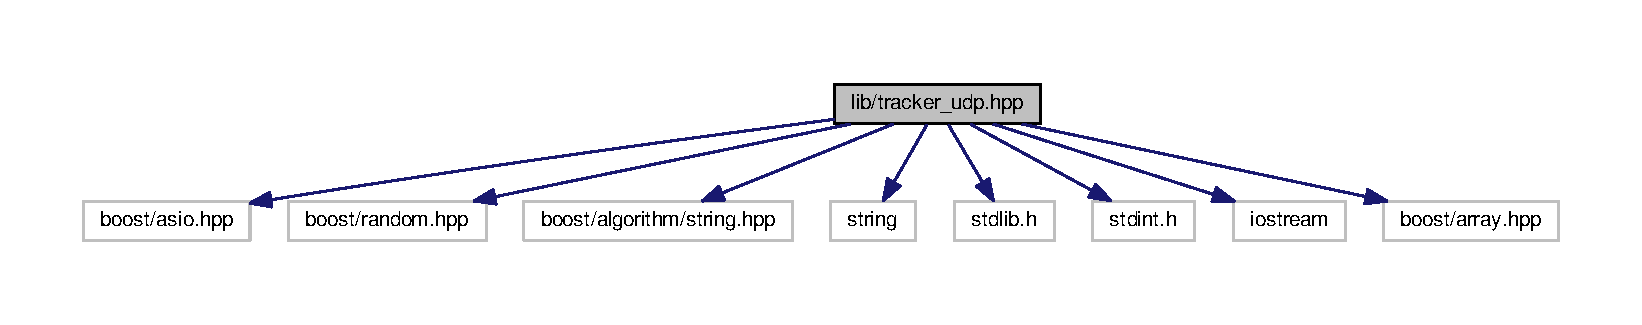
\includegraphics[width=350pt]{tracker__udp_8hpp__incl}
\end{center}
\end{figure}
\subsection*{Classes}
\begin{DoxyCompactItemize}
\item 
struct \hyperlink{structt__udp_1_1connect__request}{t\+\_\+udp\+::connect\+\_\+request}
\item 
struct \hyperlink{structt__udp_1_1connect__response}{t\+\_\+udp\+::connect\+\_\+response}
\item 
struct \hyperlink{structt__udp_1_1announce__request}{t\+\_\+udp\+::announce\+\_\+request}
\item 
struct \hyperlink{structt__udp_1_1announce__response}{t\+\_\+udp\+::announce\+\_\+response}
\end{DoxyCompactItemize}
\subsection*{Namespaces}
\begin{DoxyCompactItemize}
\item 
 \hyperlink{namespacet__udp}{t\+\_\+udp}
\end{DoxyCompactItemize}
\subsection*{Enumerations}
\begin{DoxyCompactItemize}
\item 
\mbox{\Hypertarget{namespacet__udp_a6196aec9debc020a36ee358692339614}\label{namespacet__udp_a6196aec9debc020a36ee358692339614}} 
enum {\bfseries action\+\_\+type} \{ {\bfseries none} = 0, 
{\bfseries announce} = 1, 
{\bfseries scrape} = 2, 
{\bfseries error} = 3
 \}
\end{DoxyCompactItemize}
\subsection*{Functions}
\begin{DoxyCompactItemize}
\item 
bool \hyperlink{namespacet__udp_af6fbd38370a6f5f7d8520144de7104c4}{t\+\_\+udp\+::is\+\_\+udp\+\_\+tracker} (const std\+::string \&tracker\+\_\+url)
\item 
void \hyperlink{namespacet__udp_a0e87c0151a7bceaace19434206566199}{t\+\_\+udp\+::get\+\_\+tracker\+\_\+domain} (std\+::string tracker\+\_\+url, std\+::string \&udp\+\_\+tracker, uint \&port)
\item 
void \hyperlink{namespacet__udp_af26a254f05566a7066b6930ad998a656}{t\+\_\+udp\+::udp\+\_\+manager} (const std\+::string tracker\+\_\+url, \hyperlink{structtracker_1_1TParameter}{tracker\+::\+T\+Parameter} param, pwp\+::\+Peer\+List peer\+\_\+list)
\item 
void \hyperlink{namespacet__udp_af6b2788d8ce8ab98f367838a7e3b7b09}{t\+\_\+udp\+::verify\+\_\+connect\+\_\+resp} (const std\+::vector$<$ uint8\+\_\+t $>$ \&resp, uint32\+\_\+t \&trans\+\_\+id, uint64\+\_\+t \&conn\+\_\+id, std\+::vector$<$ uint8\+\_\+t $>$ \&conn\+\_\+id\+\_\+v)
\item 
void \hyperlink{namespacet__udp_a5e968355a7c45dae0749b80e1be8308a}{t\+\_\+udp\+::get\+\_\+announce\+\_\+req} (std\+::vector$<$ uint8\+\_\+t $>$ \&req, const \hyperlink{structtracker_1_1TParameter}{tracker\+::\+T\+Parameter} \&param, std\+::vector$<$ uint8\+\_\+t $>$ \&conn\+\_\+id\+\_\+v)
\item 
void \hyperlink{namespacet__udp_a1f2a0ab9801cbc55002e67c166895a0e}{t\+\_\+udp\+::parse\+\_\+announce\+\_\+resp} (std\+::vector$<$ uint8\+\_\+t $>$ \&resp, pwp\+::\+Peer\+List peer\+\_\+list)
\item 
void \hyperlink{namespacet__udp_aab582ebbfac6fd929e811527e44384c1}{t\+\_\+udp\+::process\+\_\+error} (std\+::vector$<$ uint8\+\_\+t $>$ \&resp)
\item 
void \hyperlink{namespacet__udp_a8aa6906fdd81689928634df34688fed1}{t\+\_\+udp\+::parse\+\_\+announce\+\_\+resp\+\_\+peers} (std\+::vector$<$ uint8\+\_\+t $>$ \&resp, pwp\+::\+Peer\+List peer\+\_\+list)
\begin{DoxyCompactList}\small\item\em Peer-\/\+ID string are setted to \char`\"{}\char`\"{} since it\textquotesingle{}s not sendend with this procotol. \end{DoxyCompactList}\end{DoxyCompactItemize}


\subsection{Detailed Description}
Tracker U\+DP protocol function

Tracker U\+DP protocol messagge specification and implementation 
%--- End generated contents ---

% Index
\backmatter
\newpage
\phantomsection
\clearemptydoublepage
\addcontentsline{toc}{chapter}{Index}
\printindex

\end{document}
